% !TEX program = lualatex
% Tema 2: mismo contenido que la versión anterior; sólo cambia el formato.
\documentclass[11pt,twoside]{article}
\usepackage{apuntes-oscuro}
\usepackage[siunitx]{circuitikz}
\usepackage{subcaption}

\asignatura{Ecuaciones Diferenciales}
\cabecera{Tema 2\ \ ·\ \ Aplicaciones de las EDO de primer orden}
\hypersetup{pdftitle={Tema 2. Aplicaciones de las EDO de primer orden a modelos sencillos},
  pdfauthor={Daniel Martín Guerrero}}

% numeración de figuras y tablas global, como en la versión original
\counterwithout{figure}{section}
\counterwithout{table}{section}
\captionsetup[sub]{font=footnotesize,labelfont={color=acc},textfont={color=muted}}

% ---------- notación ----------
\newcommand\vh{\hat v}
\newcommand\xh{\hat x}
\newcommand\yhh{\hat y}
\newcommand\encab[1]{\par\addvspace{4pt}\noindent{\color{acc}\bfseries #1.}\ \ignorespaces}
\newcommand\subencab[1]{\par\addvspace{6pt}\noindent{\color{lav}\itshape #1}\par\nobreak\vspace{2pt}}
\newcommand\fin{\hfill\textcolor{muted}{$\diamond$}}
\newcommand\abs[1]{\lvert#1\rvert}
\newcommand\leyenda[2]{\textcolor{#1}{\rule[2.2pt]{11pt}{1.1pt}}\ #2}
\newcommand\leyendad[2]{\textcolor{#1}{\rule[2.2pt]{3.5pt}{1.1pt}\,\rule[2.2pt]{3.5pt}{1.1pt}}\ #2}
\pgfplotsset{t2/.style={oscuro,axis lines=left,
  every axis x label/.style={at={(axis description cs:1.0,0)},anchor=west,xshift=5pt},
  every axis y label/.style={at={(axis description cs:0,1.0)},anchor=south,yshift=3pt},samples=250}}

\begin{document}

% =====================================================================
%  PORTADA
% =====================================================================
\begin{titlepage}
\thispagestyle{empty}
\centering
\vspace*{-0.6cm}

\includegraphics[width=4.6cm]{figuras/usal.png}\par
\vspace{0.75cm}
{\color{sky}\rule{\textwidth}{0.5pt}}\par
\vspace{0.55cm}
{\color{muted}\small\textls[220]{\textsc{Facultad de Ciencias}}\quad·\quad\textls[220]{\textsc{Grado en Física}}}\par
\vspace{1.25cm}
{\color{acc}\textls[260]{\textsc{Ecuaciones Diferenciales}}}\par
\vspace{0.2cm}
{\color{muted}\small\textls[260]{\textsc{Tema 2}}}\par
\vspace{1.25cm}
{\fontsize{27}{33}\selectfont\bfseries Aplicaciones de las EDO\par}
\vspace{0.12cm}
{\fontsize{19}{24}\selectfont\bfseries de primer orden a modelos sencillos\par}
\vspace{0.55cm}
{\color{acc}\rule{2.4cm}{0.8pt}}\par
\vspace{0.45cm}
{\color{muted}\small\itshape Enfriamiento de Newton\quad·\quad Dinámica de poblaciones\quad·\quad Competición de especies\par
Fuerzas dependientes de la velocidad\quad·\quad Circuitos eléctricos\par}
\vspace{0.45cm}
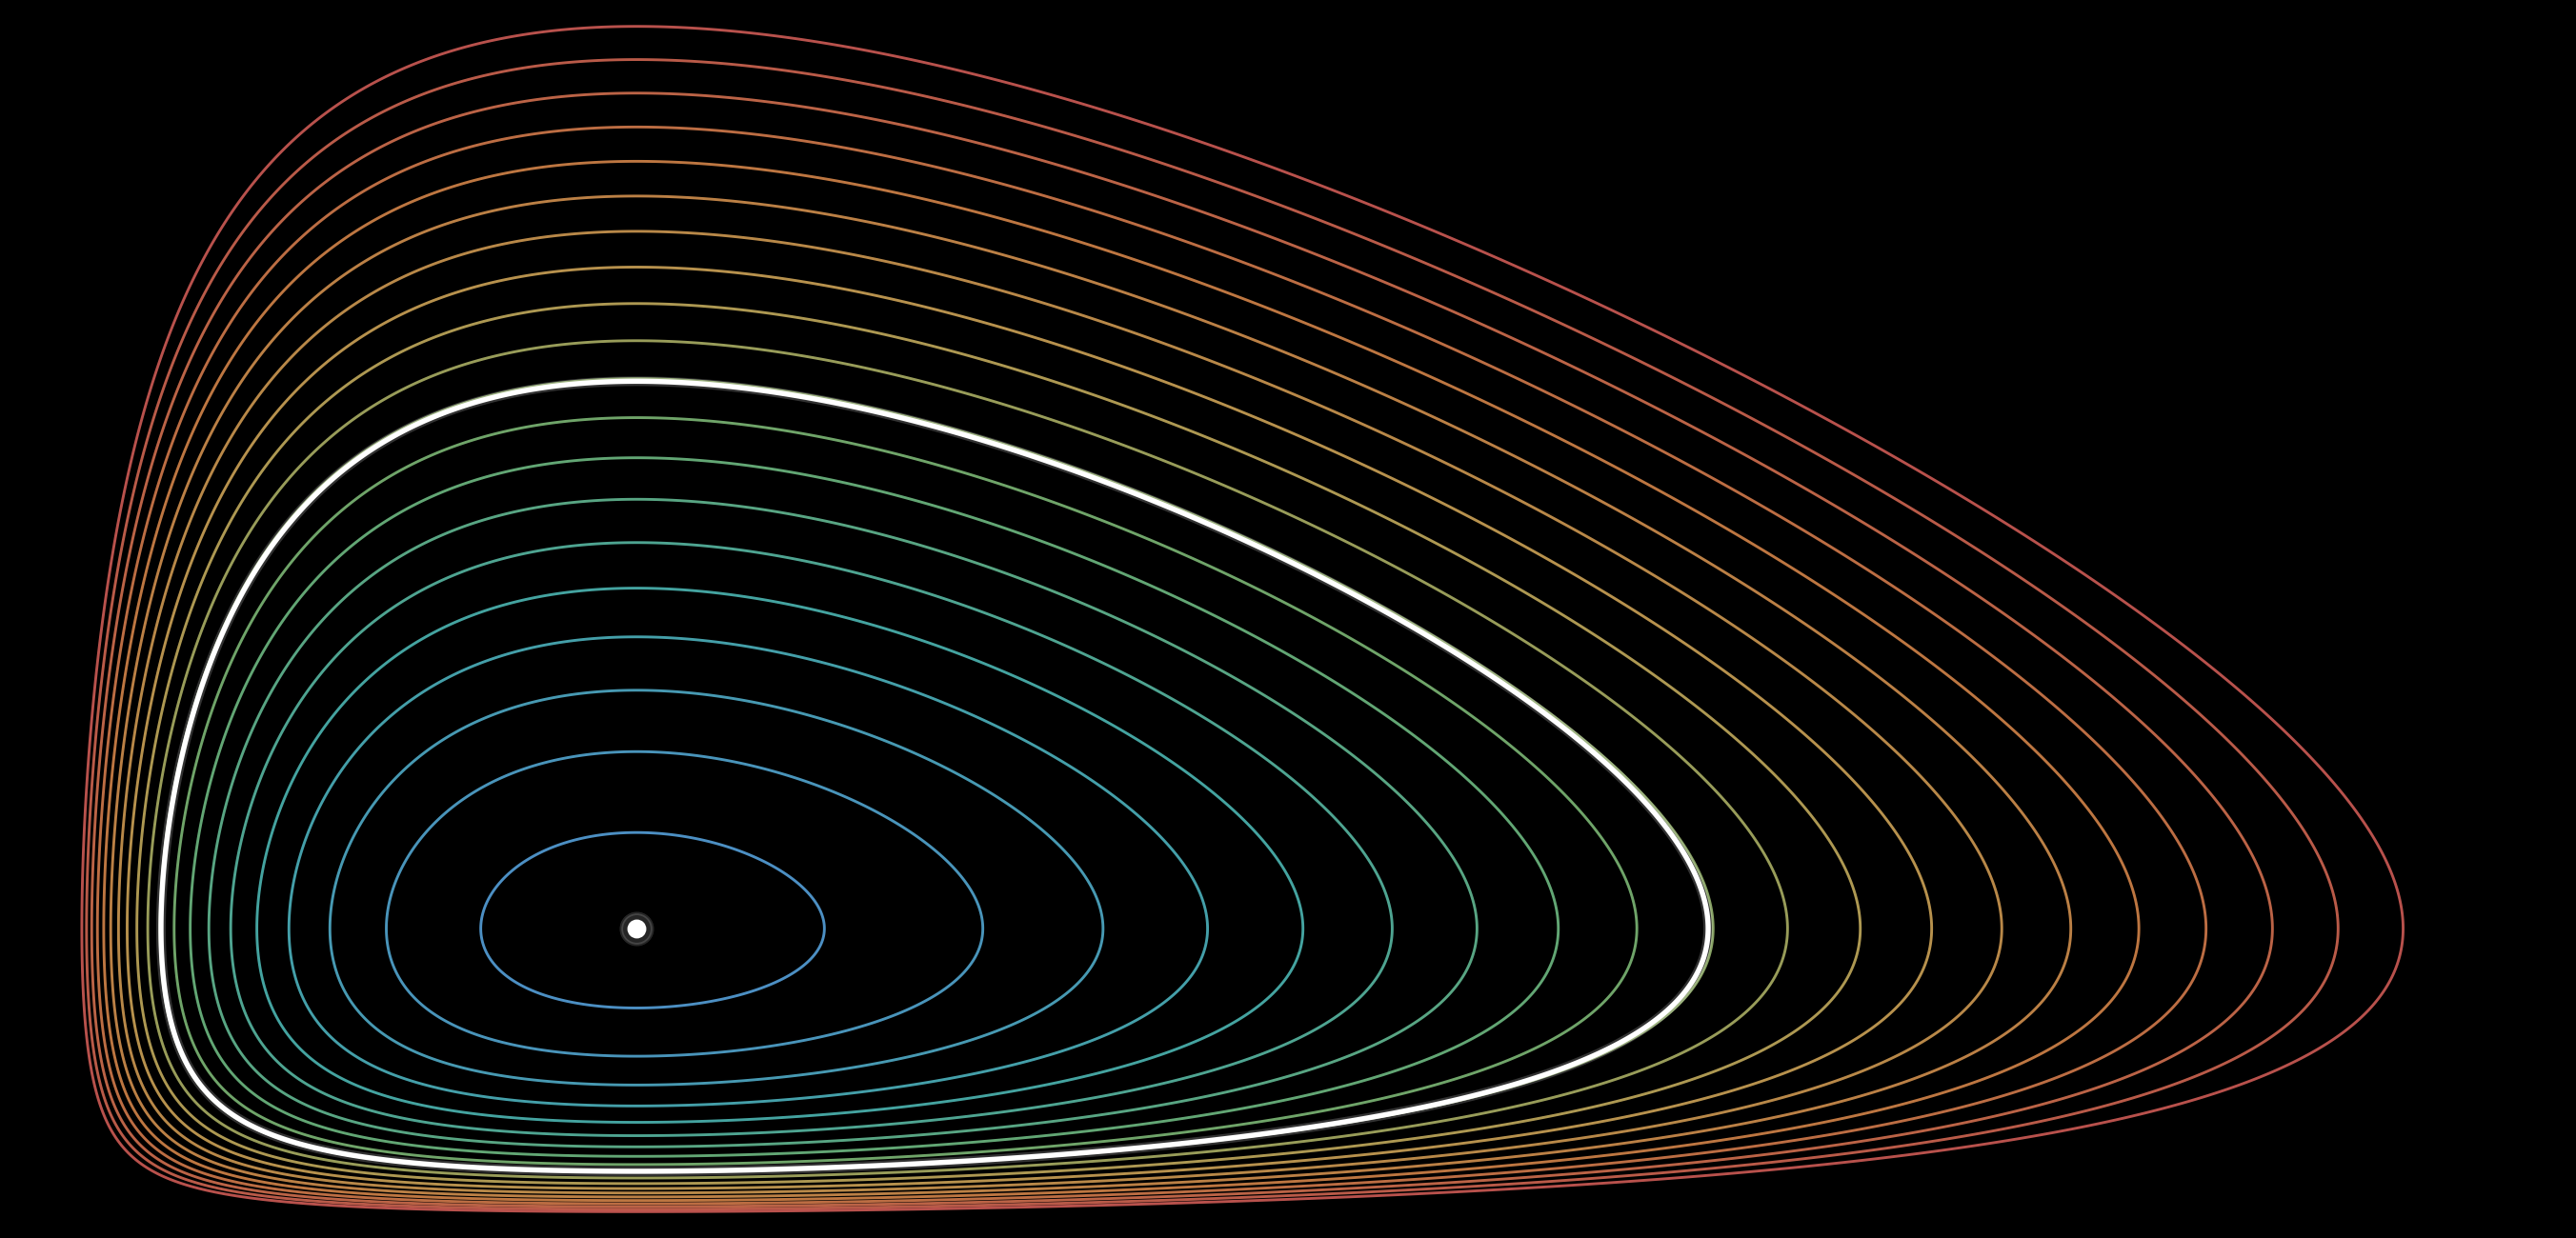
\includegraphics[width=0.86\textwidth]{figuras/portada_t2.png}\par
\vspace{0.35cm}
{\small$\displaystyle \dot x=\alpha x-\beta xy,\quad \dot y=-\gamma y+\delta xy
\quad\Longrightarrow\quad H(x,y)=\delta x-\gamma\ln x+\beta y-\alpha\ln y=c$\par}
\vfill
{\color{sky}\rule{\textwidth}{0.5pt}}\par
\vspace{0.3cm}
\begin{minipage}[t]{0.32\textwidth}\raggedright
{\color{acc}\footnotesize\textls[200]{\textsc{Autor}}}\par\vspace{2pt}
{\small Daniel Martín Guerrero}
\end{minipage}\hfill
\begin{minipage}[t]{0.32\textwidth}\centering
{\color{acc}\footnotesize\textls[200]{\textsc{Profesorado}}}\par\vspace{2pt}
{\small Pilar García Estévez\\ José Beltrán Jiménez\\ María Pérez Garrote}
\end{minipage}\hfill
\begin{minipage}[t]{0.32\textwidth}\raggedleft
{\color{acc}\footnotesize\textls[200]{\textsc{Apuntes formalizados}}}\par\vspace{2pt}
{\small Salamanca, curso 2026/2027}\\[1pt]
{\footnotesize\color{muted}Teoría y seminarios prácticos}
\end{minipage}
\end{titlepage}

\setcounter{page}{2}
{\hypersetup{linkcolor=fg}\tableofcontents}
\clearpage

% =====================================================================
\section{Ley de Newton del enfriamiento}\label{sec:newton}
% =====================================================================

\begin{motivacion}{Resumen}
Se estudian modelos de la física, la biología y la ingeniería que se reducen a ecuaciones diferenciales ordinarias de
primer orden: enfriamiento de Newton, dinámica de poblaciones, competición de especies, fuerzas dependientes de la
velocidad y circuitos eléctricos.
\end{motivacion}

La ley de Newton describe el intercambio de calor de un cuerpo con su entorno cuando domina la convección y la diferencia
de temperaturas es moderada: la temperatura del objeto varía con una velocidad proporcional a la diferencia entre su
temperatura y la del ambiente.

\begin{modelo}{enfriamiento de Newton}
Sean $T(t)$ la temperatura del objeto, $T_0=T(0)$ su temperatura inicial y $S(t)$ la temperatura ambiente (\emph{source}).
Entonces
\begin{equation}\label{eq:newton}
\dv{T}{t}=-k\big(T-S(t)\big),\qquad T(0)=T_0,
\end{equation}
con $k>0$ constante de enfriamiento. Sus dimensiones son las de una frecuencia, $[k]=[\mathrm T]^{-1}$.
\end{modelo}

\fijanum{1.1}
\begin{observacion}
Si $T>S$ entonces $\dot T<0$ y el objeto se enfría; si $T<S$ entonces $\dot T>0$ y se calienta. En ambos casos $T$
tiende a acercarse a $S$.
\end{observacion}

Reordenando términos, \eqref{eq:newton} es una ecuación lineal de primer orden con coeficiente constante:
\begin{equation}\label{eq:newtonlin}
\dot T+k\,T=k\,S(t).
\end{equation}

\fijanum{1.1}
\begin{proposicion}[solución para un ambiente arbitrario]\label{prop:newtongen}
Si $S$ es continua, la solución de \eqref{eq:newtonlin} con $T(0)=T_0$ es
\begin{equation}\label{eq:newtonsol}
T(t)=\e^{-kt}\Big[T_0+k\int_0^t\e^{ks}\,S(s)\,\dd s\Big].
\end{equation}
\end{proposicion}

\begin{demostracion}
Multiplicando \eqref{eq:newtonlin} por el factor integrante $\e^{kt}$ se obtiene
$\dfrac{\dd}{\dd t}\big(\e^{kt}T\big)=k\,\e^{kt}S(t)$. Integrando entre $0$ y $t$ y despejando $T$ se llega a \eqref{eq:newtonsol}.
\end{demostracion}

\subencab{Ambiente a temperatura constante}
Supongamos $S(t)\equiv S_0$. La ecuación \eqref{eq:newtonlin} se resuelve en dos etapas.

\fijanum{1.1}
\begin{algoritmo}[ecuación lineal $\dot y+a\,y=b(t)$]
\begin{pasosalg}
\item \emph{Homogénea.} $\dot T_h+kT_h=0$ es de variables separables: $\dd T_h/T_h=-k\,\dd t$, luego $T_h=C\,\e^{-kt}$.
\item \emph{Variación de la constante (Lagrange).} Se busca $T=C(t)\,\e^{-kt}$. Al sustituir, los términos en $C$ se
cancelan y queda $\dot C\,\e^{-kt}=kS_0$, es decir, $C(t)=S_0\,\e^{kt}+c_0$.
\item \emph{Solución general.} $T(t)=S_0+c_0\,\e^{-kt}$. Alternativamente, $T_p\equiv S_0$ se halla por inspección
(solución estacionaria, $\dot T=0$) y $T=T_h+T_p$.
\item \emph{Condición inicial.} $T(0)=T_0$ da $c_0=T_0-S_0$.
\end{pasosalg}
\end{algoritmo}

\fijanum{1.2}
\begin{proposicion}[solución con ambiente constante]\label{prop:newtonconst}
La solución del problema \eqref{eq:newton} con $S\equiv S_0$ es
\begin{equation}\label{eq:newtonconst}
\res{T(t)=S_0+(T_0-S_0)\,\e^{-kt}}
\end{equation}
y $T(t)\to S_0$ cuando $t\to\infty$.
\end{proposicion}

\begin{demostracion}
Es el resultado del algoritmo anterior. También se obtiene de \eqref{eq:newtonsol}, ya que
$k\int_0^t\e^{ks}S_0\,\dd s=S_0(\e^{kt}-1)$. Como $k>0$, el término exponencial tiende a cero.
\end{demostracion}

\fijanum{1.2}
\begin{observacion}
La magnitud $\tau=1/k$ es la \emph{constante de tiempo}: la diferencia $T-S_0$ se reduce en un factor $\e^{-1}$ cada
intervalo $\tau$. La convergencia a $S_0$ es asintótica: $T(t)=S_0$ solo en el límite $t\to\infty$ (o, a efectos
prácticos, para $t$ suficientemente grande).
\end{observacion}

\begin{figure}[!htbp]
\centering
\begin{tikzpicture}
\begin{axis}[t2,width=12.6cm,height=5.4cm,xmin=0,xmax=122,ymin=0,ymax=118,
  xtick={0,20,...,120},ytick={0,20,50,100},yticklabels={$0$,$S_0$,$50$,$100$},
  xlabel={$t$ (min)},ylabel={$T$ ($^\circ$C)}]
\addplot[muted,dashed,line width=0.5pt,domain=0:122,samples=2] {20};
\addplot[c4,domain=0:122] {20+90*exp(-0.04*x)};
\addplot[c0,domain=0:122] {20-15*exp(-0.04*x)};
\node[font=\scriptsize,anchor=west] at (axis cs:70,98) {\leyenda{c4}{enfriamiento ($T_0>S_0$)}};
\node[font=\scriptsize,anchor=west] at (axis cs:70,84) {\leyenda{c0}{calentamiento ($T_0<S_0$)}};
\end{axis}
\end{tikzpicture}
\caption{Ley de Newton con $S_0=20\,^\circ$C y $k=0.04$/min. Toda solución converge a $S_0$.}
\label{fig:newton}
\end{figure}

\fijanum{1.3}
\begin{ejemplo}
Un cuerpo a $T_0=90\,^\circ$C se sitúa en un entorno a $S_0=20\,^\circ$C. Tras $10$\,min su temperatura es $60\,^\circ$C.
Determinar $k$ y el instante en que alcanza $30\,^\circ$C.

De \eqref{eq:newtonconst}, $60=20+70\,\e^{-10k}$, luego
\begin{equation*}
k=\tfrac1{10}\ln\tfrac{70}{40}\approx0.056/\text{min}.
\end{equation*}
Imponiendo $T(t)=30$: $\e^{-kt}=\frac{10}{70}$, de donde $t=\frac1k\ln7\approx34.8$\,min.\fin
\end{ejemplo}

Cuando el ambiente varía con el tiempo, \eqref{eq:newtonsol} sigue siendo válida. Los casos $S(t)=S_0+b\sin\omega t$ y
$S(t)=S_0\,\e^{-\omega t}$ se resuelven con detalle, por varios métodos, en el apartado~\ref{sec:seminarios} (problemas 1 y 2).

% =====================================================================
\section{Dinámica de poblaciones}\label{sec:poblaciones}
% =====================================================================

Sea $P(t)$ el tamaño de una población. Los modelos de esta sección son ecuaciones autónomas $\dot P=f(P)$ con
$f(P)=P\,g(P)$, donde $g$ es la tasa de crecimiento per cápita. Los modelos difieren en la forma de $g$.

\subsection{El modelo de Malthus}

\fijanum{2.1}
\begin{definicion}[Modelo de Malthus]
La tasa de crecimiento per cápita es constante, $g\equiv k$. Para una población inicial $P(0)=P_0>0$:
\begin{equation}\label{eq:malthus}
\dv{P}{t}=kP,
\end{equation}
donde $k$ es la diferencia entre la tasa de natalidad y la de mortalidad. Es un mecanismo de control de la población.
\end{definicion}

Por separación de variables, $\int\dd P/P=\int k\,\dd t$, y por tanto
\begin{equation}\label{eq:malthussol}
P(t)=P_0\,\e^{kt}.
\end{equation}

Si $k>0$ la población crece exponencialmente (explosión demográfica), con tiempo de duplicación $t_2=\ln2/k$; si $k<0$ se
extingue exponencialmente (por ejemplo, una epidemia fatal que aniquila la población). Un crecimiento exponencial
indefinido no es realista cuando los recursos son finitos: el modelo no impone ninguna cota superior.

\subsection{El modelo logístico}

\fijanum{2.2}
\begin{definicion}[Modelo logístico (Verhulst)]
Sea $M>0$ la población máxima sostenible con los recursos disponibles. El modelo logístico es
\begin{equation}\label{eq:logistica}
\dv{P}{t}=r\,(M-P)\,P,\qquad P(0)=P_0>0,
\end{equation}
con $r>0$ relacionada con la tasa de crecimiento. Para $P\ll M$ se recupera el modelo de Malthus con $k=rM$.
\end{definicion}

La ecuación \eqref{eq:logistica} es de Riccati. Como $P\equiv0$ es una solución trivial, es además un caso particular de
ecuación de Bernoulli ($n=2$). Sus equilibrios son $P=0$ (inestable) y $P=M$ (asintóticamente estable).

\fijanum{2.1}
\begin{algoritmo}[Riccati con una solución conocida]
\begin{pasosalg}
\item Identificar una solución particular $P_1$ (aquí $P_1\equiv0$, o bien $P_1\equiv M$).
\item Sustituir $P=P_1+1/z$. Con $P_1=0$: $P=1/z$ y $\dot P=-\dot z/z^2$.
\item Resolver la ecuación lineal resultante en $z(t)$ (homogénea más solución particular).
\item Deshacer el cambio, $P=1/z$, e imponer $P(0)=P_0$.
\end{pasosalg}
\end{algoritmo}

\fijanum{2.1}
\begin{proposicion}[solución logística]\label{prop:logistica}
La solución de \eqref{eq:logistica} es
\begin{equation}\label{eq:logisticasol}
P(t)=\frac{MP_0}{P_0+(M-P_0)\,\e^{-rMt}}=\frac{M}{1+\Big(\dfrac{M}{P_0}-1\Big)\e^{-rMt}},
\end{equation}
y $P(t)\to M$ cuando $t\to\infty$ para todo $P_0>0$.
\end{proposicion}

\begin{demostracion}
Con $P=1/z$, la ecuación \eqref{eq:logistica} da
\begin{equation*}
-\frac1{z^2}\,\dot z=\frac{rM}{z}-\frac{r}{z^2}\quad\Longrightarrow\quad\dot z+rM\,z=r.
\end{equation*}
Una solución particular es $z_p=1/M$ (se comprueba: $\dot z_p=0$ y $rM/M=r$); la homogénea es $z_h=c\,\e^{-rMt}$.
Entonces $z=\frac1M+c\,\e^{-rMt}$, y $z(0)=1/P_0$ da $c=\frac1{P_0}-\frac1M$. Invirtiendo $P=1/z$:
\begin{equation*}
P=\frac{1}{\frac1M+\big(\frac1{P_0}-\frac1M\big)\e^{-rMt}}=\frac{M}{1+\big(\frac{M}{P_0}-1\big)\e^{-rMt}}.
\end{equation*}
Para $t=0$ se obtiene $P_0$ y, para $t\to\infty$, $M$.
\end{demostracion}

\fijanum{2.1}
\begin{observacion}
El modelo es autosostenible: evita la catástrofe demográfica en la que la población crece o decrece indefinidamente
(por ejemplo, durante una epidemia). Si $P_0<M$ la población crece hacia $M$ con forma sigmoidea; si $P_0>M$ decrece
monótonamente hacia $M$. Además, $\ddot P=r(M-2P)\dot P$, de modo que el punto de inflexión se sitúa en $P=M/2$.
\end{observacion}

\begin{figure}[!htbp]
\centering
\begin{tikzpicture}
\begin{axis}[t2,width=12.6cm,height=5.2cm,xmin=0,xmax=10.3,ymin=0,ymax=170,
  xtick={0,...,10},ytick={0,50,100,150},xlabel={$t$},ylabel={$P$}]
\addplot[muted,dashed,line width=0.5pt,domain=0:10.3,samples=2] {100};
\node[muted,font=\scriptsize,anchor=south west] at (axis cs:0.15,101) {$M$};
\addplot[c0,domain=0:10.3] {100/(1+9*exp(-0.8*x))};
\addplot[c4,domain=0:10.3] {100/(1-0.375*exp(-0.8*x))};
\addplot[only marks,mark=*,mark size=1.4pt,gold] coordinates {(2.7465,50)};
\node[gold,font=\scriptsize,anchor=west] at (axis cs:2.85,46) {inflexión, $P=M/2$};
\node[font=\scriptsize,anchor=west] at (axis cs:7.0,60) {\leyenda{c0}{$P_0<M$}};
\node[font=\scriptsize,anchor=west] at (axis cs:7.0,42) {\leyenda{c4}{$P_0>M$}};
\end{axis}
\end{tikzpicture}
\caption{Soluciones logísticas con $M=100$ y $rM=0.8$. Si $P_0<M$ la curva es sigmoidea; si $P_0>M$ decrece
monótonamente hacia $M$.}
\label{fig:logistica}
\end{figure}

\subsection{La ley de Gompertz}

\fijanum{2.3}
\begin{definicion}[Ley de Gompertz]
La variación de la población obedece
\begin{equation}\label{eq:gompertz}
\dv{P}{t}=b\,\big(\ln M-\ln P\big)\,P,\qquad P(0)=P_0>0,
\end{equation}
con $b>0$ y $M>0$ la población máxima sostenible.
\end{definicion}

\fijanum{2.2}
\begin{proposicion}[solución de Gompertz]\label{prop:gompertz}
La solución de \eqref{eq:gompertz} es
\begin{equation}\label{eq:gompertzsol}
P(t)=M\exp\Big[\ln\frac{P_0}{M}\,\e^{-bt}\Big],
\end{equation}
y $P(t)\to M$ cuando $t\to\infty$.
\end{proposicion}

\begin{demostracion}
Con $z=\ln P$ (es decir, $P=\e^{z}$) se tiene $\e^{z}\dot z=b(\ln M-z)\,\e^{z}$, luego
\begin{equation*}
\dot z+b\,z=b\ln M,
\end{equation*}
ecuación lineal. La solución particular es $z_p=\ln M$ y la homogénea es $z_h=c\,\e^{-bt}$, de modo que
$z=\ln M+c\,\e^{-bt}$. La condición $\ln P(0)=\ln P_0$ da $c=\ln P_0-\ln M=\ln(P_0/M)$. Equivalentemente,
$\ln(P/M)=\ln(P_0/M)\,\e^{-bt}$, y $\ln(M/P)=\ln(M/P_0)\,\e^{-bt}$. Deshaciendo el cambio se obtiene \eqref{eq:gompertzsol}.
Para $t=0$ se tiene $P=P_0$ y para $t\to\infty$, $P=M$.
\end{demostracion}

\fijanum{2.3}
\begin{lema}[punto de inflexión]\label{lem:gompertz}
Si $P_0<M/\e$, la solución \eqref{eq:gompertzsol} tiene un único punto de inflexión, en $P_i=M/\e$, que corresponde al
instante $t_i$ tal que $\e^{bt_i}=\ln(M/P_0)$.
\end{lema}

\begin{demostracion}
Derivando \eqref{eq:gompertz},
\begin{equation*}
\ddot P=b\,\dot P\ln\frac MP-b\,\dot P=b\,\dot P\Big(\ln\frac MP-1\Big).
\end{equation*}
Como $\dot P>0$ para $0<P<M$, $\ddot P=0$ si y solo si $\ln(M/P)=1$, es decir, $P=M/\e$. Con \eqref{eq:gompertzsol},
$\ln(M/P)=\ln(M/P_0)\,\e^{-bt}=1$ da el instante $t_i$.
\end{demostracion}

La población crece rápidamente hasta $P_i=M/\e\approx0.37\,M$ y, a partir de ese punto, atenúa el crecimiento. Al igual
que en la logística, el sistema es autosostenible, pero el crecimiento deja de ser simétrico: el punto de inflexión aparece
antes que en la logística ($M/2$). La derivada temporal $\dot P$ da la velocidad de crecimiento y presenta un máximo en el
punto de inflexión.

\fijanum{2.2}
\begin{observacion}[aplicaciones de la ley de Gompertz]
\begin{itemize}
\item \emph{Adopción de tecnologías} (por ejemplo, teléfonos móviles): los costes iniciales son altos y la aceptación es
lenta; sigue un periodo de crecimiento rápido y, por último, una disminución de la absorción cuando se alcanza la saturación.
\item \emph{Población en un espacio cerrado}: la tasa de natalidad aumenta y luego el crecimiento se ralentiza conforme se
alcanza el límite de los recursos.
\item \emph{Crecimiento de tumores}.
\end{itemize}
\end{observacion}

\begin{figure}[!htbp]
\centering
\begin{subfigure}[b]{0.48\textwidth}\centering
\begin{tikzpicture}
\begin{axis}[t2,width=6.9cm,height=5.0cm,xmin=0,xmax=10.3,ymin=0,ymax=112,
  xtick={0,2,...,10},ytick={0,50,100},xlabel={$t$},ylabel={$P$}]
\addplot[muted,dashed,line width=0.5pt,domain=0:10.3,samples=2] {100};
\addplot[c0,domain=0:10.3] {100*exp(ln(1/50)*exp(-0.5*x))};
\addplot[c2,domain=0:10.3] {100*exp(ln(1/5)*exp(-0.5*x))};
\addplot[c3,domain=0:10.3] {100*exp(ln(1/2)*exp(-0.5*x))};
\node[font=\scriptsize,anchor=west] at (axis cs:5.3,46) {\leyenda{c0}{$P_0/M=\frac1{50}$}};
\node[font=\scriptsize,anchor=west] at (axis cs:5.3,31) {\leyenda{c2}{$P_0/M=\frac15$}};
\node[font=\scriptsize,anchor=west] at (axis cs:5.3,16) {\leyenda{c3}{$P_0/M=\frac12$}};
\end{axis}
\end{tikzpicture}
\caption{Soluciones de Gompertz ($M=100$, $b=0.5$).}
\end{subfigure}\hfill
\begin{subfigure}[b]{0.48\textwidth}\centering
\begin{tikzpicture}
\begin{axis}[t2,width=6.9cm,height=5.0cm,xmin=0,xmax=10.3,ymin=0,ymax=112,
  xtick={0,2,...,10},ytick={0,50,100},xlabel={$t$},ylabel={$P$}]
\addplot[muted,dashed,line width=0.5pt,domain=0:10.3,samples=2] {100};
\addplot[c0,domain=0:10.3] {100*exp(ln(1/20)*exp(-0.5*x))};
\addplot[c4,domain=0:10.3] {100/(1+19*exp(-0.55*x))};
\addplot[only marks,mark=*,mark size=1.5pt,c0] coordinates {(2.1948,36.788)};
\addplot[only marks,mark=square*,mark size=1.4pt,c4] coordinates {(5.3534,50)};
\node[c0,font=\scriptsize,anchor=south east] at (axis cs:2.05,39) {$M/\e$};
\node[c4,font=\scriptsize,anchor=north west] at (axis cs:5.5,48) {$M/2$};
\node[font=\scriptsize,anchor=west] at (axis cs:6.6,31) {\leyenda{c0}{Gompertz}};
\node[font=\scriptsize,anchor=west] at (axis cs:6.6,16) {\leyenda{c4}{logística}};
\end{axis}
\end{tikzpicture}
\caption{Comparación con la logística; se indican los puntos de inflexión.}
\end{subfigure}
\caption{Ley de Gompertz. Las trayectorias convergen a $M$; la inflexión ocurre en $P=M/\e$ (Gompertz) frente a
$P=M/2$ (logística).}
\label{fig:gompertz}
\end{figure}

\subsection{Curvas de infección SIS}

Sea $N$ el número de individuos de una población, dividida en susceptibles $S(t)$ (que pueden contraer la infección) e
infectados $I(t)$. Los infectados se recuperan y vuelven a ser susceptibles: no hay inmunidad permanente.

\begin{modelo}{SIS}
\begin{equation}\label{eq:sis}
\dot S=-\beta SI+\gamma I,\qquad\dot I=\beta SI-\gamma I,
\end{equation}
con $\beta>0$ la tasa de contagio (número de personas a las que puede infectar cada infectado, por unidad de tiempo) y
$\gamma>0$ la tasa de recuperación; $1/\gamma$ es el periodo medio de infección. Se cumple $\dot S+\dot I=0$, luego $S+I=N$.
\end{modelo}

Sustituyendo $S=N-I$ el sistema se reduce a una única ecuación de Riccati (de nuevo con $I\equiv0$ como solución):
\begin{equation}\label{eq:sisI}
\dot I=\big[\beta(N-I)-\gamma\big]I=(\beta N-\gamma)\,I-\beta I^2,\qquad I(0)=I_0.
\end{equation}
Se define $k=N-\gamma/\beta$, de modo que $\beta N-\gamma=\beta k$, y el \emph{número reproductivo básico} $R_0=\beta N/\gamma$,
que cumple $R_0>1\iff k>0$.

\fijanum{2.4}
\begin{teorema}[curva de infección SIS]\label{teo:sis}
Sea $I_0\in(0,N]$. Para $k\neq0$, la solución de \eqref{eq:sisI} es
\begin{equation}\label{eq:sissol}
I(t)=\frac{k}{1+\Big(\dfrac{k}{I_0}-1\Big)\e^{-\beta kt}}.
\end{equation}
Si $R_0>1$ ($k>0$), $I(t)\to k$ cuando $t\to\infty$, con $k$ independiente de $I_0$; si $R_0<1$ ($k<0$), $I(t)\to0$. Si
$R_0=1$, $I(t)=I_0/(1+\beta I_0t)\to0$.
\end{teorema}

\begin{demostracion}
Con $I=1/z$ se obtiene
\begin{equation*}
-\frac1{z^2}\,\dot z=\frac{\beta N-\gamma}{z}-\frac{\beta}{z^2}\quad\Longrightarrow\quad\dot z+\beta k\,z=\beta.
\end{equation*}
La solución particular es $z_p=1/k$ y la homogénea es $c\,\e^{-\beta kt}$: $z=\frac1k+c\,\e^{-\beta kt}$. Para $t=0$,
$\frac1{I_0}=\frac1k+c$, luego $c=\frac1{I_0}-\frac1k=\frac{k-I_0}{kI_0}$. Invirtiendo, $I=1/z=k\big/\big(1+kc\,\e^{-\beta kt}\big)$,
que es \eqref{eq:sissol}. El comportamiento asintótico se sigue del signo de $k$ en el exponente. Para $k=0$, $\dot z=\beta$ y
$z=1/I_0+\beta t$.
\end{demostracion}

\fijanum{2.3}
\begin{observacion}
Si $0<I_0<k$ la curva crece hasta $k$; si $I_0>k>0$ decrece hasta $k$. El caso de interés epidemiológico es $0<I_0<k$ (un
pequeño inóculo en una población con $R_0>1$). El valor $k=N-\gamma/\beta$ es el número de infectados que persisten una vez
alcanzado el régimen estacionario (endémico).
\end{observacion}

La derivada $\dot I=\beta I(k-I)$ es la velocidad con la que se propaga la epidemia. Alcanza su máximo cuando $I=k/2$.

\fijanum{2.5}
\begin{proposicion}[pico de la velocidad de propagación]\label{prop:pico}
Si $0<I_0<k/2$, la velocidad $\dot I(t)$ es máxima en
\begin{equation}\label{eq:pico}
t^*=\frac1{k\beta}\ln\Big(\frac{k}{I_0}-1\Big).
\end{equation}
\end{proposicion}

\begin{demostracion}
$\ddot I=\beta(k-2I)\dot I$ se anula si $I=k/2$. De \eqref{eq:sissol}, $I(t^*)=k/2$ equivale a
$\big(\frac k{I_0}-1\big)\e^{-\beta kt^*}=1$, que da \eqref{eq:pico}. Si $I_0\ge k/2$, $\dot I$ es decreciente desde $t=0$.
\end{demostracion}

\begin{figure}[!htbp]
\centering
\begin{subfigure}[b]{0.48\textwidth}\centering
\begin{tikzpicture}
\begin{axis}[t2,width=6.9cm,height=5.0cm,xmin=0,xmax=2.08,ymin=0,ymax=2.15,
  xtick={0,0.5,1,1.5,2},ytick={0,0.3,1,1.7,2},yticklabels={$0$,$N\!-\!k$,$1$,$k$,$2$},xlabel={$t$},ylabel={$I,\,S$}]
\addplot[muted,dashed,line width=0.5pt,domain=0:2.08,samples=2] {1.7};
\addplot[muted,dashed,line width=0.5pt,domain=0:2.08,samples=2] {0.3};
\addplot[c0,domain=0:2.08] {1.7/(1+(1.7/0.5-1)*exp(-1.7*x))};
\addplot[c2,domain=0:2.08] {1.7/(1+(1.7/1-1)*exp(-1.7*x))};
\addplot[c3,domain=0:2.08] {1.7/(1+(1.7/1.5-1)*exp(-1.7*x))};
\addplot[c0,dashed,domain=0:2.08] {2-1.7/(1+(1.7/0.5-1)*exp(-1.7*x))};
\addplot[c2,dashed,domain=0:2.08] {2-1.7/(1+(1.7/1-1)*exp(-1.7*x))};
\addplot[c3,dashed,domain=0:2.08] {2-1.7/(1+(1.7/1.5-1)*exp(-1.7*x))};
\end{axis}
\end{tikzpicture}
\caption{Infectados $I(t)$ (crecientes, continuo) y susceptibles $S=N-I$ (decrecientes, discontinuo).}
\end{subfigure}\hfill
\begin{subfigure}[b]{0.48\textwidth}\centering
\begin{tikzpicture}
\begin{axis}[t2,width=6.9cm,height=5.0cm,xmin=0,xmax=2.08,ymin=0,ymax=0.82,
  xtick={0,0.5,1,1.5,2},ytick={0,0.2,0.4,0.6,0.8},xlabel={$t$},ylabel={$\dot I$}]
\addplot[c0,domain=0:2.08] {(1.7/(1+2.4*exp(-1.7*x)))*(1.7-1.7/(1+2.4*exp(-1.7*x)))};
\addplot[c2,domain=0:2.08] {(1.7/(1+0.7*exp(-1.7*x)))*(1.7-1.7/(1+0.7*exp(-1.7*x)))};
\addplot[c3,domain=0:2.08] {(1.7/(1+0.13333*exp(-1.7*x)))*(1.7-1.7/(1+0.13333*exp(-1.7*x)))};
\addplot[only marks,mark=*,mark size=1.5pt,gold] coordinates {(0.51498,0.7225)};
\node[gold,font=\scriptsize,anchor=south] at (axis cs:0.515,0.735) {$t^*$};
\end{axis}
\end{tikzpicture}
\caption{Velocidad de propagación $\dot I$; el pico para $I_0=\frac12$ se da en $t^*$.}
\end{subfigure}\\[4pt]
{\scriptsize\leyenda{c0}{$I_0=\frac12$}\qquad\leyenda{c2}{$I_0=1$}\qquad\leyenda{c3}{$I_0=\frac32$}}
\caption{Modelo SIS con $N=2$, $\beta=1$, $\gamma=0.3$ (de modo que $k=1.7$). El valor $k$ es independiente de $I_0$.}
\label{fig:sis}
\end{figure}

\subsection{Extensión: modelo SIR}

En una enfermedad con inmunidad, o con mortalidad, hay que contar una variable más (por ejemplo, los recuperados o
fallecidos), lo que exige modelos con más compartimentos. El más sencillo es el modelo SIR:
\begin{equation}\label{eq:sir}
\dot S=-\beta SI,\qquad\dot I=\beta SI-\gamma I,\qquad\dot R=\gamma I,
\end{equation}
con $S+I+R=N$ y $R_0=\beta N/\gamma$. Aquí $R(t)$ son los individuos retirados (recuperados inmunes o fallecidos).

\fijanum{2.6}
\begin{proposicion}[integral primera del modelo SIR]\label{prop:sir}
Las trayectorias en el plano de fases $(S,I)$ verifican
\begin{equation}\label{eq:sirint}
I+S-\frac\gamma\beta\ln S=I_0+S_0-\frac\gamma\beta\ln S_0,
\end{equation}
y el número de infectados es máximo cuando $S=\gamma/\beta=N/R_0$. Si $R_0>1$ y $I_0\ll N$, el valor máximo es
\begin{equation}\label{eq:imax}
I_{\max}\simeq N\Big[1-\frac{1+\ln R_0}{R_0}\Big].
\end{equation}
\end{proposicion}

\begin{demostracion}
De \eqref{eq:sir}, $\dfrac{\dd I}{\dd S}=-1+\dfrac{\gamma}{\beta S}$, que es separable y da \eqref{eq:sirint}. El máximo de $I$
ocurre cuando $\dot I=0$ con $I>0$, es decir, $S=\gamma/\beta$. Sustituyendo en \eqref{eq:sirint} con $S_0\simeq N$ e
$I_0\simeq0$ se obtiene \eqref{eq:imax}.
\end{demostracion}

\fijanum{2.4}
\begin{observacion}
Para $R_0=4$ y $N=10^4$ resulta $I_{\max}\simeq4034$ personas, en $S=N/R_0=2500$. Además, la epidemia termina con un número
de susceptibles $S_\infty>0$ que no se contagian (aquí $S_\infty\simeq198$): la enfermedad se extingue por falta de
infectados, no de susceptibles.
\end{observacion}

\begin{figure}[!htbp]
\centering
\begin{subfigure}[b]{0.48\textwidth}\centering
\begin{tikzpicture}
\begin{axis}[t2,width=6.9cm,height=5.0cm,xmin=0,xmax=205,ymin=0,ymax=10800,
  xtick={0,50,100,150,200},ytick={0,5000,10000},yticklabels={$0$,$5000$,$10^4$},
  scaled y ticks=false,xlabel={$t$},ylabel={personas}]
\addplot[c0,sharp plot] table[x=t,y=S] {figuras/datos/t2_sir4.dat};
\addplot[c5,sharp plot] table[x=t,y=I] {figuras/datos/t2_sir4.dat};
\addplot[c2,sharp plot] table[x=t,y=R] {figuras/datos/t2_sir4.dat};
\node[c0,font=\scriptsize,anchor=west] at (axis cs:60,1300) {$S$};
\node[c5,font=\scriptsize,anchor=west] at (axis cs:42,4100) {$I$};
\node[c2,font=\scriptsize,anchor=north] at (axis cs:120,9600) {$R$};
\end{axis}
\end{tikzpicture}
\caption{Evolución temporal ($R_0=4$).}
\end{subfigure}\hfill
\begin{subfigure}[b]{0.48\textwidth}\centering
\begin{tikzpicture}
\begin{axis}[t2,width=6.9cm,height=5.0cm,xmin=0,xmax=205,ymin=0,ymax=4500,
  xtick={0,50,100,150,200},ytick={0,1000,2000,3000,4000},scaled y ticks=false,xlabel={$t$},ylabel={$I$}]
\addplot[c0,sharp plot] table[x=t,y=a] {figuras/datos/t2_sirR0.dat};
\addplot[c2,sharp plot] table[x=t,y=b] {figuras/datos/t2_sirR0.dat};
\addplot[c3,sharp plot] table[x=t,y=c] {figuras/datos/t2_sirR0.dat};
\addplot[c5,sharp plot] table[x=t,y=d] {figuras/datos/t2_sirR0.dat};
\node[font=\scriptsize,anchor=west] at (axis cs:118,4050) {\leyenda{c0}{$R_0=0.8$}};
\node[font=\scriptsize,anchor=west] at (axis cs:118,3600) {\leyenda{c2}{$R_0=1.5$}};
\node[font=\scriptsize,anchor=west] at (axis cs:118,3150) {\leyenda{c3}{$R_0=2.5$}};
\node[font=\scriptsize,anchor=west] at (axis cs:118,2700) {\leyenda{c5}{$R_0=4$}};
\end{axis}
\end{tikzpicture}
\caption{Comparación de $R_0$ ($\gamma=0.1$).}
\end{subfigure}\\[8pt]
\begin{subfigure}[b]{0.9\textwidth}\centering
\begin{tikzpicture}
\begin{axis}[t2,width=11.2cm,height=6.0cm,xmin=0,xmax=10400,ymin=0,ymax=10400,
  xtick={0,2500,5000,7500,10000},ytick={0,5000,10000},yticklabels={$0$,$5000$,$10^4$},
  xticklabels={$0$,\textcolor{gold}{$N/R_0$},$5000$,$7500$,$10^4$},scaled ticks=false,
  xlabel={$S$},ylabel={$I$}]
\fill[muted,opacity=0.13] (axis cs:0,10000) -- (axis cs:10000,0) -- (axis cs:10400,0) -- (axis cs:10400,10400) -- (axis cs:0,10400) -- cycle;
\draw[muted,line width=0.4pt,dashed] (axis cs:0,10000) -- (axis cs:10000,0);
\addplot[muted,line width=0.45pt,-{Stealth[length=3pt,width=2.6pt]},
  quiver={u=\thisrow{u},v=\thisrow{v}}] table[x=S,y=I] {figuras/datos/t2_sircampo.dat};
\addplot[c5,line width=1.0pt,sharp plot] table[x=S,y=I] {figuras/datos/t2_sirfase.dat};
\addplot[only marks,mark=*,mark size=1.6pt,gold] coordinates {(2500,4034)};
\node[gold,font=\scriptsize,anchor=south] at (axis cs:2500,4150) {$I_{\max}$};
\draw[gold,line width=0.4pt,dashed] (axis cs:2500,0) -- (axis cs:2500,4034);

\node[muted,font=\scriptsize] at (axis cs:7800,7600) {$S+I>N$};
\end{axis}
\end{tikzpicture}
\caption{Plano de fases $(S,I)$ ($R_0=4$): campo de direcciones y trayectoria. La zona gris, $S+I>N$, es inaccesible.}
\end{subfigure}
\caption{Modelo SIR para una pandemia con $N=10^4$, $\gamma=0.1$ e $I_0=1$.}
\label{fig:sir}
\end{figure}

% =====================================================================
\section{Competición de especies}\label{sec:competicion}
% =====================================================================

\subsection{Modelos de Lotka--Volterra (equilibrio ecológico)}

Consideremos dos especies que interactúan como presa y depredador: los conejos (presa), cuya población es $x(t)$, y los
zorros (depredador), con población $y(t)$. Los conejos se reproducen mucho más rápido que los zorros.

\begin{modelo}{Lotka--Volterra}
\begin{equation}\label{eq:lv}
\dot x=\alpha x-\beta xy,\qquad\dot y=-\gamma y+\delta xy,
\end{equation}
con $\alpha,\beta,\gamma,\delta>0$. Los términos $\alpha x$ y $-\gamma y$ son las tasas de reproducción (crecimiento de las
presas sin depredadores y decaimiento de los depredadores sin presas), y los términos $\mp xy$ describen la interacción: es
mala para los conejos que haya zorros, y buena para los zorros que haya conejos.
\end{modelo}

Dividiendo las dos ecuaciones se elimina el tiempo y se obtiene la ecuación de las órbitas:
\begin{equation}\label{eq:lvorb}
\dv{y}{x}=\frac{y\,(\delta x-\gamma)}{x\,(\alpha-\beta y)},
\end{equation}
que es de variables separables. Separando,
\begin{equation*}
\frac{\alpha-\beta y}{y}\,\dd y=\frac{\delta x-\gamma}{x}\,\dd x\iff\Big(\frac\alpha y-\beta\Big)\dd y+\Big(\frac\gamma x-\delta\Big)\dd x=0.
\end{equation*}
La forma de Pfaff resultante es exacta, y se integra directamente:
\begin{equation}\label{eq:lvH}
\alpha\ln y-\beta y+\gamma\ln x-\delta x=\text{cte}\quad\iff\quad H(x,y)\equiv\delta x-\gamma\ln x+\beta y-\alpha\ln y=c.
\end{equation}
La constante se determina con las condiciones iniciales de población: $c=H(x_0,y_0)$.

\fijanum{3.1}
\begin{teorema}[órbitas cerradas]\label{teo:lv}
El sistema \eqref{eq:lv} tiene dos equilibrios: $(0,0)$, que es un punto de silla, y $(x^*,y^*)=(\gamma/\delta,\,\alpha/\beta)$.
La función $H$ es una integral primera, y sus conjuntos de nivel $\{H=c\}$ en el primer cuadrante, con $c>H(x^*,y^*)$, son
curvas cerradas que rodean a $(x^*,y^*)$. Por tanto, toda solución con $x_0,y_0>0$ distinta del equilibrio es periódica.
\end{teorema}

\begin{demostracion}
A lo largo de las soluciones,
\begin{equation*}
\dot H=\Big(\delta-\frac\gamma x\Big)\dot x+\Big(\beta-\frac\alpha y\Big)\dot y=(\delta x-\gamma)(\alpha-\beta y)+(\beta y-\alpha)(\delta x-\gamma)=0.
\end{equation*}
Además, $\nabla H=0$ solo en $(x^*,y^*)$, donde la matriz hessiana $\diag(\gamma/x^2,\,\alpha/y^2)$ es definida positiva, y
$H\to+\infty$ cuando $(x,y)$ se aproxima a la frontera del primer cuadrante o a infinito. Luego $(x^*,y^*)$ es el único mínimo
de $H$ y los conjuntos de nivel son compactos y simples, es decir, curvas cerradas. Como no contienen equilibrios, la
solución las recorre periódicamente.
\end{demostracion}

\begin{desarrollo}{las cuatro fases del ciclo}
Las rectas $x=x^*$ e $y=y^*$ dividen el plano en cuatro regiones, según el signo de $\dot x=x(\alpha-\beta y)$ y de
$\dot y=y(\delta x-\gamma)$. Una órbita se recorre en sentido antihorario:
\begin{itemize}
\item[\textbf{(I)}] $x>x^*$, $y<y^*$: $\dot x>0$, $\dot y>0$. Aumentan conejos y zorros.
\item[\textbf{(II)}] $x>x^*$, $y>y^*$: $\dot x<0$, $\dot y>0$. Los zorros se comen a los conejos, que disminuyen.
\item[\textbf{(III)}] $x<x^*$, $y>y^*$: $\dot x<0$, $\dot y<0$. Hay pocos conejos y los zorros pasan hambre.
\item[\textbf{(IV)}] $x<x^*$, $y<y^*$: $\dot x>0$, $\dot y<0$. Como hay menos zorros, los conejos pueden reproducirse mejor.
\end{itemize}
Estos son los llamados \emph{ciclos ecológicos}: ninguna de las especies desaparece.
\end{desarrollo}

\fijanum{3.1}
\begin{observacion}[principio de Volterra]
Si $T$ es el periodo, integrando $\dot y/y=-\gamma+\delta x$ sobre un ciclo se obtiene $0=-\gamma T+\delta\int_0^Tx\,\dd t$.
Las poblaciones medias son, por tanto, $\langle x\rangle=\gamma/\delta$ y $\langle y\rangle=\alpha/\beta$, es decir, las del equilibrio.
\end{observacion}

\begin{figure}[!htbp]
\centering
\begin{subfigure}[b]{0.48\textwidth}\centering
\begin{tikzpicture}
\begin{axis}[t2,width=6.9cm,height=6.3cm,xmin=0,xmax=4.0,ymin=0,ymax=4.0,axis equal image,
  xtick={0,1,2,3},ytick={0,1,2,3},xticklabels={$0$,$x^*$,$2$,$3$},yticklabels={$0$,$y^*$,$2$,$3$},
  xlabel={$x$},ylabel={$y$},
  every axis x label/.style={at={(axis description cs:1.0,0)},anchor=north west,xshift=-6pt,yshift=-3pt}]
\draw[muted,line width=0.4pt,dashed] (axis cs:1,0) -- (axis cs:1,3.95);
\draw[muted,line width=0.4pt,dashed] (axis cs:0,1) -- (axis cs:3.95,1);
\addplot[c0,sharp plot,line width=0.9pt,postaction={decorate},decoration={markings,mark=at position 0.62 with {\arrow{Stealth[length=5pt]}}},sharp plot] table[x=x,y=y] {figuras/datos/t2_lv_23.dat};
\addplot[c3,sharp plot,line width=0.9pt,postaction={decorate},decoration={markings,mark=at position 0.62 with {\arrow{Stealth[length=5pt]}}},sharp plot] table[x=x,y=y] {figuras/datos/t2_lv_28.dat};
\addplot[c5,sharp plot,line width=0.9pt,postaction={decorate},decoration={markings,mark=at position 0.62 with {\arrow{Stealth[length=5pt]}}},sharp plot] table[x=x,y=y] {figuras/datos/t2_lv_34.dat};
\addplot[only marks,mark=*,mark size=1.6pt,fg] coordinates {(1,1)};

\node[font=\scriptsize,lav] at (axis cs:1.3,0.75) {I};
\node[font=\scriptsize,lav] at (axis cs:1.3,1.25) {II};
\node[font=\scriptsize,lav] at (axis cs:0.72,1.25) {III};
\node[font=\scriptsize,lav] at (axis cs:0.72,0.75) {IV};
\end{axis}
\end{tikzpicture}
\caption{Órbitas $H=c$ ($c=2.3;\ 2.8;\ 3.4$), con el sentido de recorrido y las cuatro fases.}
\end{subfigure}\hfill
\begin{subfigure}[b]{0.48\textwidth}\centering
\begin{tikzpicture}
\begin{axis}[t2,width=6.9cm,height=6.3cm,xmin=0,xmax=14.3,ymin=0,ymax=3.55,
  xtick={0,5,10},ytick={0,1,2,3},xlabel={$t$},ylabel={población}]
\addplot[c3,sharp plot] table[x=t,y=x] {figuras/datos/t2_lv_tiempo.dat};
\addplot[c0,dashed,sharp plot] table[x=t,y=y] {figuras/datos/t2_lv_tiempo.dat};
\node[font=\scriptsize,anchor=west] at (axis cs:0.4,3.38) {\leyenda{c3}{$x$ (presas)}};
\node[font=\scriptsize,anchor=west] at (axis cs:6.6,3.38) {\leyendad{c0}{$y$ (depredadores)}};
\end{axis}
\end{tikzpicture}
\caption{Evolución temporal ($c=2.8$): oscilaciones desfasadas.}
\end{subfigure}
\caption{Modelo de Lotka--Volterra con $\alpha=\beta=\gamma=\delta=1$. Las órbitas, recorridas en sentido antihorario, son
curvas cerradas (ciclos ecológicos) alrededor del equilibrio $(1,1)$.}
\label{fig:lv}
\end{figure}

\subsection{Curvas de persecución}\label{sec:persecucion}

Un conejo se mueve en línea recta y un zorro intenta alcanzarlo, dirigiéndose en cada instante hacia él.

\begin{modelo}{persecución}
Se toma el eje $y$ como la recta a lo largo de la cual se mueve el conejo con velocidad constante $\vh$, partiendo del
origen. Su posición es $\hat{\bm r}=(\xh,\yhh)$ con
\begin{equation}\label{eq:conejo}
\xh=0,\qquad\yhh=\vh\,t.
\end{equation}
El zorro parte de $(a,0)$ y corre con velocidad $v$, constante en módulo pero no en dirección. Su posición es
$\bm r=(x,y)$, con
\begin{equation}\label{eq:zorro}
x(0)=a,\qquad y(0)=0,\qquad\dot{\bm r}(0)=-v\,\hat{\bm\imath}.
\end{equation}
En todo instante, la velocidad del zorro apunta hacia el conejo.
\end{modelo}

\begin{figure}[!htbp]
\centering
\begin{tikzpicture}
\begin{axis}[t2,width=11cm,height=5.8cm,xmin=0,xmax=1.12,ymin=0,ymax=0.78,clip=false,
  xtick={0.42,1},xticklabels={$x$,$a$},ytick={0.2973},yticklabels={$\vh t$},xlabel={$x$},ylabel={$y$}]
\addplot[fg,line width=0.9pt,domain=0.002:1,samples=250] {0.5*((x^1.5)/1.5-(x^0.5)/0.5)+0.5/0.75};
\draw[muted,line width=0.4pt,dashed] (axis cs:0.42,0) -- (axis cs:0.42,0.1093);
\draw[gold,line width=0.7pt,dashed] (axis cs:0,0.2973) -- (axis cs:0.42,0.1093);
\draw[c0,line width=0.9pt,-{Stealth[length=6pt]}] (axis cs:0.42,0.1093) -- (axis cs:0.2374,0.191);
\draw[c3,line width=0.9pt,-{Stealth[length=6pt]}] (axis cs:0,0.2973) -- (axis cs:0,0.47);
\addplot[only marks,mark=*,mark size=1.6pt,fg] coordinates {(0.42,0.1093) (1,0)};
\addplot[only marks,mark=square*,mark size=1.6pt,c3] coordinates {(0,0.2973)};
\node[c0,font=\scriptsize,anchor=north] at (axis cs:0.33,0.13) {$\bm v$};
\node[c3,font=\scriptsize,anchor=east] at (axis cs:-0.01,0.44) {$\vh$};
\node[fg,font=\scriptsize,anchor=south west] at (axis cs:0.43,0.115) {$(x,y)$};
\node[gold,font=\scriptsize,anchor=north west] at (axis cs:0.03,0.145) {línea de visión};
\draw[gold,line width=0.4pt,-{Stealth[length=3pt]}] (axis cs:0.095,0.15) -- (axis cs:0.115,0.232);
\node[fg,font=\scriptsize,anchor=south] at (axis cs:1,0.025) {zorro};
\node[c3,font=\scriptsize,anchor=east] at (axis cs:-0.01,0.36) {conejo};
\end{axis}
\end{tikzpicture}
\caption{Geometría de la persecución ($k=1/2$). La velocidad del zorro es tangente a su trayectoria y apunta al conejo, de
modo que $y'=-(\yhh-y)/x$.}
\label{fig:persecuciongeo}
\end{figure}

\begin{desarrollo}{ecuación de la trayectoria del zorro}
Sea $y'=\dd y/\dd x$.
\begin{pasos}
\item \emph{Módulo de la velocidad.} $v^2=\dot x^2+\dot y^2=\dot x^2(1+y'^2)$. Como $x$ decrece con $t$, $\dot x<0$ y
\begin{equation}\label{eq:pers1}
v\,\dd t=-\sqrt{1+y'^2}\,\dd x.
\end{equation}
\item \emph{Dirección.} El zorro corre hacia el conejo: $y'=-\dfrac{\yhh-y}{x}=-\dfrac{\vh t-y}{x}$, es decir,
\begin{equation}\label{eq:pers2}
\vh\,t=y-x\,y'.
\end{equation}
\item \emph{Eliminación del tiempo.} Diferenciando \eqref{eq:pers2} respecto a $x$: $\vh\,\dd t=\big(y'-y'-xy''\big)\dd x=-x\,y''\,\dd x$.
Con \eqref{eq:pers1}, y llamando $k=\vh/v$,
\begin{equation}\label{eq:pers3}
x\,y''=k\sqrt{1+y'^2},\qquad k=\frac{\vh}{v}.
\end{equation}
\item \emph{Reducción de orden.} Como $y$ no aparece explícitamente, se toma $z=y'$ y queda la ecuación de primer orden separable
\begin{equation*}
x\,z'=k\sqrt{1+z^2}\quad\Longrightarrow\quad\frac{\dd z}{\sqrt{1+z^2}}=k\,\frac{\dd x}{x}.
\end{equation*}
\end{pasos}
\end{desarrollo}

\fijanum{3.2}
\begin{lema}[una primitiva elemental]\label{lem:primitiva}
\begin{equation*}
\int\frac{\dd z}{\sqrt{1+z^2}}=\ln\Big(z+\sqrt{1+z^2}\Big)+C.
\end{equation*}
\end{lema}

\begin{demostracion}
Se hace la sustitución trigonométrica $z=\tan\theta$, de modo que $\dd z=\sec^2\theta\,\dd\theta$ y
$\sqrt{1+z^2}=\sqrt{1+\tan^2\theta}=\sec\theta$. Entonces
\begin{equation*}
\int\frac{\sec^2\theta}{\sec\theta}\,\dd\theta=\int\sec\theta\,\dd\theta=\ln\abs{\sec\theta+\tan\theta}+C=\ln\Big(\sqrt{1+z^2}+z\Big)+C.
\end{equation*}
(Para integrandos con $\sqrt{a^2-x^2}$, $\sqrt{a^2+x^2}$ o $\sqrt{x^2-a^2}$ se toman, respectivamente, $x=a\sin\theta$,
$x=a\tan\theta$ o $x=a\sec\theta$.)
\end{demostracion}

Integrando, $\ln\big(y'+\sqrt{1+y'^2}\big)-k\ln x=C$. En $x=a$ se tiene $y'=0$, luego $C=-k\ln a$ y
\begin{equation}\label{eq:pers4}
y'+\sqrt{1+y'^2}=\Big(\frac xa\Big)^{k}.
\end{equation}
Despejamos $y'$. Aislando la raíz, $\sqrt{1+y'^2}=(x/a)^k-y'$, y elevando al cuadrado, $1=(x/a)^{2k}-2y'(x/a)^k$. De donde
\begin{equation}\label{eq:pers5}
y'=\frac{(x/a)^{2k}-1}{2(x/a)^k}=\frac12\Big[\Big(\frac xa\Big)^{k}-\Big(\frac xa\Big)^{-k}\Big].
\end{equation}
(Equivalentemente: $\sqrt{1+y'^2}-y'=(x/a)^{-k}$, y se resta o suma a \eqref{eq:pers4}.)

\fijanum{3.3}
\begin{teorema}[trayectoria del zorro]\label{teo:zorro}
Si $k=\vh/v<1$, la trayectoria del zorro es
\begin{equation}\label{eq:pers6}
y(x)=\frac a2\Big[\frac1{1+k}\Big(\frac xa\Big)^{1+k}-\frac1{1-k}\Big(\frac xa\Big)^{1-k}\Big]+\frac{ak}{1-k^2},
\end{equation}
y el zorro alcanza al conejo en $x=0$, en el instante $t_{\mathrm f}=\dfrac{av}{v^2-\vh^2}$, en la posición
$\yhh_f=y_f=\dfrac{av\vh}{v^2-\vh^2}$.
\end{teorema}

\begin{demostracion}
Se integra \eqref{eq:pers5} con $u=x/a$, $\dd x=a\,\dd u$:
\begin{equation*}
y=\frac a2\Big(\int u^{k}\,\dd u-\int u^{-k}\,\dd u\Big)=\frac a2\Big[\frac{u^{1+k}}{1+k}-\frac{u^{1-k}}{1-k}\Big]+C_1,
\end{equation*}
válido para $k\neq1$. La condición $y(a)=0$ ($u=1$) da $C_1=\dfrac a2\Big[\dfrac1{1-k}-\dfrac1{1+k}\Big]=\dfrac{ak}{1-k^2}$, lo
que prueba \eqref{eq:pers6}.

Si $k<1$ el exponente $1-k$ es positivo, de modo que al llegar a $x=0$ los dos primeros términos se anulan y
$y(0)=\dfrac{ak}{1-k^2}$. El zorro y el conejo coinciden cuando $x=\xh=0$ e $y=\yhh$: $\dfrac{ak}{1-k^2}=\vh\,t_{\mathrm f}$. Con
$k=\vh/v$,
\begin{equation*}
t_{\mathrm f}=\frac{ak}{\vh(1-k^2)}=\frac av\cdot\frac1{1-\vh^2/v^2}=\frac{av}{v^2-\vh^2},\qquad
\yhh_f=\vh\,t_{\mathrm f}=\frac{av\vh}{v^2-\vh^2}.
\end{equation*}
\end{demostracion}

\fijanum{3.2}
\begin{observacion}
Si $k>1$ ($\vh>v$) el término $-(x/a)^{1-k}/(1-k)$ diverge al hacer $x\to0$, y el zorro nunca alcanza al conejo. El caso
límite $k=1$ (misma velocidad) se trata en el problema 6 del apartado~\ref{sec:seminarios}: el zorro tampoco lo alcanza y la
distancia mínima es $a/2$.
\end{observacion}

\begin{figure}[!htbp]
\centering
\begin{tikzpicture}
\begin{axis}[t2,width=12cm,height=5.2cm,xmin=0,xmax=1.04,ymin=0,ymax=0.74,
  xtick={0,0.2,0.4,0.6,0.8,1},ytick={0,0.2,0.4,0.6},xlabel={$x/a$},ylabel={$y/a$}]
\addplot[c0,domain=0:1,samples=250] {0.5*((x^(1.5))/1.5-(x^(0.5))/0.5)+0.5/0.75};
\addplot[c2,domain=0:1,samples=250] {0.5*((x^(4/3))/(4/3)-(x^(2/3))/(2/3))+(1/3)/(8/9)};
\addplot[c4,domain=0:1,samples=250] {0.5*((x^(1.25))/1.25-(x^(0.75))/0.75)+0.25/(15/16)};
\addplot[only marks,mark=*,mark size=1.6pt,c0] coordinates {(0,0.6667)};
\addplot[only marks,mark=*,mark size=1.6pt,c2] coordinates {(0,0.375)};
\addplot[only marks,mark=*,mark size=1.6pt,c4] coordinates {(0,0.2667)};
\node[font=\scriptsize,anchor=west] at (axis cs:0.66,0.62) {\leyenda{c0}{$v=2\vh$}};
\node[font=\scriptsize,anchor=west] at (axis cs:0.66,0.52) {\leyenda{c2}{$v=3\vh$}};
\node[font=\scriptsize,anchor=west] at (axis cs:0.66,0.42) {\leyenda{c4}{$v=4\vh$}};
\end{axis}
\end{tikzpicture}
\caption{Curvas de persecución del zorro para distintas velocidades relativas, con $a=1$. Los puntos sobre el eje son las
posiciones de captura $y_f/a=k/(1-k^2)$.}
\label{fig:persecucion}
\end{figure}

\fijanum{3.3}
\begin{ejemplo}
Con $a=100$\,m, $\vh=5$\,m/s y $v=10$\,m/s se tiene $k=1/2$, y $t_{\mathrm f}=av/(v^2-\vh^2)=13.3$\,s, con el conejo
recorrido $\yhh_f=\vh\,t_{\mathrm f}=66.7$\,m.\fin
\end{ejemplo}

% =====================================================================
\section{Fuerzas dependientes de la velocidad}\label{sec:fuerzas}
% =====================================================================

Una partícula de masa $m$ que se mueve en una dimensión bajo una fuerza que solo depende de la velocidad, $F=F(v)$, queda
descrita por la segunda ley de Newton. Ejemplos son el arrastre lineal, $F=-bv$ (bajas velocidades), y el arrastre
cuadrático, $F=-Bv^2$ (altas velocidades).

\begin{modelo}{movimiento con $F=F(v)$}
Hay que resolver las dos ecuaciones de primer orden
\begin{align}
m\,\dv{v}{t}&=F(v),\label{eq:fv1}\\
\dv{x}{t}&=v(t).\label{eq:fv2}
\end{align}
Equivalen a la ecuación de segundo orden $m\ddot x=F(\dot x)$, de modo que la solución general $x=\varphi(t,c_1,c_2)$ depende
de dos constantes. Estas se determinan con dos condiciones iniciales: $x(t_0)=x_0=\varphi(t_0,c_1,c_2)$ y
$\dot x(t_0)=v_0=\varphi'(t_0,c_1,c_2)$.
\end{modelo}

\fijanum{4.1}
\begin{algoritmo}[movimiento con $F=F(v)$]
\begin{pasosalg}
\item \emph{Velocidad.} Separar variables en \eqref{eq:fv1}: $\displaystyle\int\frac{\dd v}{F(v)}=\int\frac{\dd t}{m}$. Esto da
$t=t(v)$ y, al invertir, $v=v(t)$ (constante $c_1$).
\item \emph{Posición.} Integrar $\dd x=v(t)\,\dd t$, es decir, $x=x(t)$ (constante $c_2$).
\item \emph{Condiciones iniciales.} Imponer $v(t_0)=v_0$ y $x(t_0)=x_0$.
\item \emph{Variante (si interesa $x$ y no $t$).} Con la regla de la cadena, $\dot v=\dfrac{\dd v}{\dd x}\dfrac{\dd x}{\dd t}=v\dfrac{\dd v}{\dd x}$,
y \eqref{eq:fv1} se escribe $m\,v\,\dd v=F(v)\,\dd x$, ecuación de variables separables que relaciona $x$ y $v$.
\end{pasosalg}
\end{algoritmo}

\fijanum{4.1}
\begin{ejemplo}[arrastre lineal, $F(v)=-kv$]
Consideramos un movimiento horizontal sin otras fuerzas, con $v(0)=v_0$. Separando variables,
\begin{equation*}
m\,\dv{v}{t}=-kv\quad\Longrightarrow\quad\frac{\dd v}{v}=-\frac km\,\dd t.
\end{equation*}
Si $v(t_f)=v_f<v_0$ (la partícula frena), integrando entre $0$ y $t_f$:
\begin{equation*}
\int_{v_0}^{v_f}\frac{\dd v}{v}=-\frac km\int_0^{t_f}\dd t\quad\Longrightarrow\quad\ln\frac{v_f}{v_0}=-\frac km\,t_f
\quad\Longrightarrow\quad t_f(v_f)=-\frac mk\ln\frac{v_f}{v_0}.
\end{equation*}
Como $v_f/v_0<1$, $\ln(v_f/v_0)<0$ y $t_f>0$. Aplicando la exponencial a ambos lados de la ecuación logarítmica,
$v_f/v_0=\e^{-kt_f/m}$, es decir,
\begin{equation}\label{eq:arrastrelin}
v(t)=v_0\,\e^{-kt/m}.
\end{equation}
La velocidad decrece exponencialmente y tiende a cero, aunque no se anula en tiempo finito. La posición se obtiene
integrando \eqref{eq:fv2}:
\begin{equation*}
x(t)=x_0+\frac{mv_0}{k}\big(1-\e^{-kt/m}\big)\longrightarrow x_0+\frac{mv_0}{k}\qquad(t\to\infty),
\end{equation*}
de modo que la distancia total recorrida es finita, $mv_0/k$.\fin
\end{ejemplo}

\fijanum{4.2}
\begin{ejemplo}[arrastre cuadrático, $F(v)=-Bv^2$]
De $m\,\dd v/v^2=-B\,\dd t$ se obtiene $1/v=1/v_0+Bt/m$, es decir,
\begin{equation*}
v(t)=\frac{v_0}{1+Bv_0t/m},\qquad x(t)=x_0+\frac mB\ln\Big(1+\frac{Bv_0t}{m}\Big).
\end{equation*}
La velocidad decae como $1/t$ y el recorrido diverge logarítmicamente. Con la variante del algoritmo:
$m\,v\,\dd v/\dd x=-Bv^2$ da $\dd v/v=-(B/m)\,\dd x$ y $v=v_0\,\e^{-B(x-x_0)/m}$.\fin
\end{ejemplo}

El caso $F=-k/v^2$, en el que la partícula se detiene en tiempo finito, se resuelve con las dos variantes del algoritmo en
el problema 3 del apartado~\ref{sec:seminarios}.

\begin{figure}[!htbp]
\centering
\begin{tikzpicture}
\begin{axis}[t2,width=12.6cm,height=5.0cm,xmin=0,xmax=3.08,ymin=0,ymax=1.08,
  xtick={0,0.5,1,1.5,2,2.5,3},ytick={0,0.5,1},xlabel={$t$},ylabel={$v/v_0$}]
\addplot[c0,domain=0:3.08] {exp(-x)};
\addplot[c3,domain=0:3.08] {1/(1+x)};
\addplot[c5,domain=0:0.33333,samples=300] {(1-3*x)^(1/3)};
\addplot[only marks,mark=*,mark size=1.5pt,c5] coordinates {(0.33333,0)};
\node[c5,font=\scriptsize,anchor=south west] at (axis cs:0.36,0.02) {$t=\frac{mv_0^3}{3k}$};
\node[font=\scriptsize,anchor=west] at (axis cs:1.9,0.95) {\leyenda{c0}{$F=-kv$}};
\node[font=\scriptsize,anchor=west] at (axis cs:1.9,0.82) {\leyenda{c3}{$F=-Bv^2$}};
\node[font=\scriptsize,anchor=west] at (axis cs:1.9,0.69) {\leyenda{c5}{$F=-k/v^2$}};
\end{axis}
\end{tikzpicture}
\caption{Frenado con distintas fuerzas dependientes de la velocidad ($m=k=B=v_0=1$). Con $F=-k/v^2$ la partícula se detiene
en el instante finito $t=mv_0^3/(3k)$.}
\label{fig:frenado}
\end{figure}

% =====================================================================
\section{Circuitos eléctricos}\label{sec:circuitos}
% =====================================================================

Consideremos un circuito con una resistencia $R$ y una autoinducción $L$ conectadas en serie con una fuente de tensión $U(t)$.

\begin{figure}[!htbp]
\centering
\begin{circuitikz}[color=fg,line width=0.6pt,scale=1.0,transform shape]
\draw[color=fg] (0,0) to[sV,l=$U(t)$,color=c0] (0,2.6)
  -- (3.6,2.6) to[L,l=$L$,i>^=$I(t)$,color=c3] (3.6,0)
  to[R,l=$R$,color=gold] (0,0);
\end{circuitikz}
\caption{Circuito $RL$ en serie con una fuente de tensión $U(t)$.}
\label{fig:circuito}
\end{figure}

\begin{modelo}{segunda ley de Kirchhoff}
La intensidad $I(t)$ que circula por el circuito cumple
\begin{equation}\label{eq:kirchhoff}
U(t)=R\,I+L\,\dv{I}{t},
\end{equation}
donde $U(t)$ es la diferencia de potencial aplicada. Equivale a la ecuación lineal $\dot I+\dfrac RL\,I=\dfrac{U(t)}{L}$, de
la forma $\dot I+a(t)I=b(t)$.
\end{modelo}

\fijanum{5.1}
\begin{observacion}[análisis dimensional]
De $[RI]=[L\dot I]$ se obtiene $[R]=[L]/[\mathrm T]$, de modo que $[R/L]=[\mathrm T]^{-1}$ tiene dimensiones de frecuencia.
La constante de tiempo del circuito es $\tau=L/R$.
\end{observacion}

\subencab{Descarga exponencial de la batería}
Tomemos $U(t)=U_0\,\e^{-\alpha t}$, con $[\alpha]=[\mathrm T]^{-1}$ (dimensiones de frecuencia). La ecuación a resolver es
\begin{equation}\label{eq:rl}
RI+L\dv{I}{t}=U_0\,\e^{-\alpha t}\iff\dot I+\frac RL\,I=\frac{U_0}{L}\,\e^{-\alpha t},\qquad I(0)=0.
\end{equation}

\fijanum{5.1}
\begin{proposicion}[corriente en el circuito $RL$]\label{prop:rl}
Si $\alpha\neq R/L$, la solución de \eqref{eq:rl} es
\begin{equation}\label{eq:rlsol}
I(t)=\frac{U_0}{R-\alpha L}\Big(\e^{-\alpha t}-\e^{-(R/L)t}\Big).
\end{equation}
Si $\alpha=R/L$ (resonancia), la solución es
\begin{equation}\label{eq:rlres}
I(t)=\frac{U_0}{L}\,t\,\e^{-(R/L)t}.
\end{equation}
\end{proposicion}

\begin{demostracion}
\emph{Homogénea.} $\dot I_h+\frac RL I_h=0$ da $\dd I_h/I_h+\frac RL\,\dd t=0$, luego $\ln I_h+\frac RL t=\text{cte}$ e
$I_h=c_0\,\e^{-(R/L)t}$.

\emph{Variación de la constante (Lagrange), $\alpha\neq R/L$.} Se busca $I_p=\kappa(t)\,\e^{-(R/L)t}$. Al sustituir se cancelan
los términos en $\kappa$ y queda
\begin{equation*}
\dot\kappa\,\e^{-(R/L)t}=\frac{U_0}{L}\,\e^{-\alpha t}\quad\Longrightarrow\quad\dot\kappa=\frac{U_0}{L}\,\e^{(R/L-\alpha)t}
\quad\Longrightarrow\quad\kappa=\frac{U_0}{L}\,\frac{\e^{(R/L-\alpha)t}}{R/L-\alpha}.
\end{equation*}
Por tanto, $I_p=\dfrac{U_0}{L(R/L-\alpha)}\,\e^{-\alpha t}=\dfrac{U_0}{R-\alpha L}\,\e^{-\alpha t}$, y la solución general es
$I=c_0\,\e^{-(R/L)t}+\dfrac{U_0}{R-\alpha L}\,\e^{-\alpha t}$. La condición $I(0)=0$ da $c_0=-\dfrac{U_0}{R-\alpha L}$, es
decir, \eqref{eq:rlsol}. La integración solo es posible si $\alpha\neq R/L$.

\emph{Caso $\alpha=R/L$.} Ahora $\dot\kappa=U_0/L$, luego $\kappa=U_0t/L+c_0$, y $I(0)=0$ da $c_0=0$, es decir, \eqref{eq:rlres}.
\end{demostracion}

\fijanum{5.2}
\begin{observacion}[resonancia]
En el caso $\alpha=R/L$ la constante de atenuación del estímulo externo coincide con la constante de relajación natural del
circuito, $R/L$. Como el término forzante $\e^{-\alpha t}$ ya es solución de la homogénea, la respuesta se amplifica
transitoriamente por un factor lineal $t$, antes de que el decaimiento exponencial acabe por disipar la energía del sistema.
La intensidad es máxima en $t=L/R$, con $I_{\max}=U_0/(\e R)$. Para $\alpha\to R/L$ se puede llegar a \eqref{eq:rlres} como
límite de \eqref{eq:rlsol}, con la regla de L'Hôpital o con un desarrollo de Taylor (problema 4 del apartado~\ref{sec:seminarios}).
\end{observacion}

\fijanum{5.3}
\begin{observacion}[batería constante]
Si $\alpha\to0$ en \eqref{eq:rlsol} se obtiene $I(t)=\dfrac{U_0}{R}\big(1-\e^{-Rt/L}\big)$, que tiende al valor de Ohm,
$U_0/R$, con constante de tiempo $\tau=L/R$.
\end{observacion}

\begin{figure}[!htbp]
\centering
\begin{tikzpicture}
\begin{axis}[t2,width=12.6cm,height=5.0cm,xmin=0,xmax=8.2,ymin=0,ymax=0.8,
  xtick={0,...,8},ytick={0,0.2,0.4,0.6},xlabel={$t$},ylabel={$I$}]
\addplot[c0,domain=0:8.2] {(exp(-0.25*x)-exp(-x))/0.75};
\addplot[c2,domain=0:8.2] {(exp(-0.5*x)-exp(-x))/0.5};
\addplot[c3,line width=1.2pt,domain=0:8.2] {x*exp(-x)};
\addplot[c5,domain=0:8.2] {(exp(-2*x)-exp(-x))/(-1)};
\addplot[only marks,mark=*,mark size=1.5pt,c3] coordinates {(1,0.3679)};
\node[font=\scriptsize,anchor=west] at (axis cs:5.0,0.72) {\leyenda{c0}{$\alpha=\frac14\frac RL$}};
\node[font=\scriptsize,anchor=west] at (axis cs:6.6,0.72) {\leyenda{c2}{$\alpha=\frac12\frac RL$}};
\node[font=\scriptsize,anchor=west] at (axis cs:5.0,0.6) {\leyenda{c3}{$\alpha=\frac RL$}};
\node[font=\scriptsize,anchor=west] at (axis cs:6.6,0.6) {\leyenda{c5}{$\alpha=2\frac RL$}};
\end{axis}
\end{tikzpicture}
\caption{Intensidad en el circuito $RL$ con $U=U_0\,\e^{-\alpha t}$ ($R/L=1$, $U_0/L=1$). En resonancia ($\alpha=R/L$) la
respuesta es $t\,\e^{-t}$, con máximo en $t=L/R$.}
\label{fig:rl}
\end{figure}

% =====================================================================
\section{Seminarios prácticos}\label{sec:seminarios}
% =====================================================================

Esta sección reúne los problemas del Tema~2 resueltos con detalle y, siempre que es posible, por varios métodos. La
tabla~\ref{tab:metodos} resume las técnicas empleadas en el tema.

\begin{table}[!htbp]
\centering
\small
\renewcommand\arraystretch{1.3}
\begin{tabular}{@{}p{3.7cm} p{5.4cm} p{3.6cm}@{}}
\toprule
\textcolor{acc}{Método} & \textcolor{acc}{Idea} & \textcolor{acc}{Dónde}\\
\midrule
Variables separables & $f(y)\,\dd y=g(x)\,\dd x$ & Malthus, Gompertz, §\ref{sec:poblaciones}\\
Ecuación lineal: factor integrante & $\e^{\int a}$ hace exacta $y'+a\,y=b$ & Newton, circuitos\\
Variación de la constante (Lagrange) & $y=C(x)\,y_h$ & Newton, circuitos\\
Coeficientes indeterminados & ensayo $y_p$ de la forma del término forzante; si hay solapamiento con $y_h$, se multiplica por $t$ & Problemas 1 y 2\\
Forma de Pfaff y factor integrante & $\mu$ tal que $\mu\omega$ sea exacta & Problema 2, ejemplo final\\
Riccati / Bernoulli & $P=1/z$ lo linealiza & logística, SIS\\
Regla de la cadena & $\dot v=v\,\dd v/\dd x$ & Problema 3\\
Reducción de orden & $z=y'$ cuando $y$ no aparece & persecución\\
Límites indeterminados & L'Hôpital, desarrollo de Taylor & Problema 4\\
\bottomrule
\end{tabular}
\caption{Métodos de resolución utilizados en el Tema~2.}
\label{tab:metodos}
\end{table}

\subsection{Enunciados}

\fijanum{6.1}
\begin{enunciado}
Resolver la ecuación de Newton del enfriamiento en el caso de que la temperatura ambiente evolucione en la forma
$S(t)=S_0+b\sin(\omega t)$.
\end{enunciado}
\fijanum{6.2}
\begin{enunciado}
Resolver la ecuación de Newton del enfriamiento en el caso de que la temperatura ambiente evolucione en la forma
$S(t)=S_0\,\e^{-\omega t}$.
\end{enunciado}
\fijanum{6.3}
\begin{enunciado}
Determinar la distancia que recorre hasta pararse un móvil de velocidad inicial $v_0$ sometido a una fuerza dependiente de
la velocidad $F=-k/v^2$.
\end{enunciado}
\fijanum{6.4}
\begin{enunciado}
Determinar la evolución temporal de la intensidad en un circuito con resistencia $R$ y autoinducción $L$ con fuerza
electromotriz $U=U_0\,\e^{-\omega t}$ cuando $\omega\to R/L$.
\end{enunciado}
\fijanum{6.5}
\begin{enunciado}
Los elementos radiactivos se desintegran a una tasa proporcional a la cantidad de elemento presente. Proponer un modelo
matemático y resolverlo utilizando como parámetros la cantidad inicial de elemento y el periodo de vida media.
\end{enunciado}
\fijanum{6.6}
\begin{enunciado}
Demostrar que un zorro que persigue a un conejo yendo a la misma velocidad que él nunca lo alcanza. Si la distancia inicial
entre ambos es $a$, demostrar que la mínima distancia entre ambos es $a/2$.
\end{enunciado}

\subsection{Soluciones}

\subsubsection*{Problema 1: ambiente oscilante $S(t)=S_0+b\sin\omega t$}

\emph{Solución.} La ley de Newton $\dot T=-k\big(T-S(t)\big)$ se reordena como la ecuación lineal
\begin{equation}\label{eq:p1}
\dot T+kT=kS_0+kb\sin\omega t.
\end{equation}

\encab{Método A: coeficientes indeterminados}\emph{Homogénea.} $\dot T_h+kT_h=0$ da $\dd T_h/T_h+k\,\dd t=0$,
$\ln T_h+kt=c$, luego $T_h=C\,\e^{-kt}$.

\emph{Solución particular.} El término no homogéneo es una constante más una función periódica, así que se propone una
solución de la misma naturaleza (sin confundir las constantes con $C$):
\begin{equation*}
T_p=A+B\sin\omega t+D\cos\omega t,\qquad\dot T_p=B\omega\cos\omega t-D\omega\sin\omega t.
\end{equation*}
Sustituyendo en \eqref{eq:p1} y agrupando por tipo de función:
\begin{equation*}
\underbrace{kA}_{\text{cte.}}+(B\omega+kD)\cos\omega t+(-D\omega+kB)\sin\omega t=kS_0+kb\sin\omega t.
\end{equation*}
Igualando coeficientes:
\begin{equation*}
A=S_0,\qquad B\omega+kD=0\ \Rightarrow\ D=-\frac\omega k\,B,\qquad-D\omega+kB=kb.
\end{equation*}
Sustituyendo $D$ en la tercera: $B\big(\frac{\omega^2}{k}+k\big)=kb$, es decir, $B\,\frac{k^2+\omega^2}{k}=kb$, y por tanto
\begin{equation*}
B=\frac{k^2b}{k^2+\omega^2},\qquad D=-\frac{k\omega b}{k^2+\omega^2}.
\end{equation*}
Sumando la homogénea, la solución general es
\begin{equation}\label{eq:p1gen}
T(t)=C\,\e^{-kt}+S_0+\frac{kb}{k^2+\omega^2}\big[k\sin\omega t-\omega\cos\omega t\big].
\end{equation}
Con $T(0)=T_0$: $T_0=C+S_0-\dfrac{k\omega b}{k^2+\omega^2}$, de donde $C=T_0-S_0+\dfrac{k\omega b}{k^2+\omega^2}$ y
\begin{equation}\label{eq:p1sol}
\res{T(t)=S_0+\Big(T_0-S_0+\frac{k\omega b}{k^2+\omega^2}\Big)\e^{-kt}+\frac{kb}{k^2+\omega^2}\big[k\sin\omega t-\omega\cos\omega t\big]}
\end{equation}

\encab{Método B: factor integrante}Con la proposición~\ref{prop:newtongen},
$T=\e^{-kt}\big[T_0+k\int_0^t\e^{ks}(S_0+b\sin\omega s)\,\dd s\big]$. Usando
\begin{equation*}
\int\e^{ks}\sin\omega s\,\dd s=\frac{\e^{ks}\,(k\sin\omega s-\omega\cos\omega s)}{k^2+\omega^2}
\end{equation*}
(se obtiene integrando por partes dos veces), se llega de nuevo a \eqref{eq:p1sol}.

\encab{Forma amplitud--fase}Como $k\sin\omega t-\omega\cos\omega t=\sqrt{k^2+\omega^2}\,\sin(\omega t-\varphi)$ con
$\tan\varphi=\omega/k$, el régimen estacionario es
\begin{equation*}
T_p(t)=S_0+\frac{b\,k}{\sqrt{k^2+\omega^2}}\,\sin(\omega t-\varphi):
\end{equation*}
el objeto oscila con la frecuencia del ambiente, con amplitud atenuada por $k/\sqrt{k^2+\omega^2}<1$ y retardado en fase en
$\varphi$. El transitorio $\e^{-kt}$ decae con constante de tiempo $1/k$.

\encab{Enfriamiento rápido}Si $\omega/k\ll1$ (el cuerpo se equilibra mucho más rápido de lo que cambia el ambiente),
$\varphi\to0$, la atenuación tiende a $1$ y el coeficiente $k\omega b/(k^2+\omega^2)\to0$. La solución se aproxima por
\begin{equation*}
T\approx S_0+(T_0-S_0)\,\e^{-kt}+b\sin\omega t,
\end{equation*}
es decir, el cuerpo sigue a la temperatura ambiente $S(t)$ tras un breve transitorio.\fin

\begin{figure}[!htbp]
\centering
\begin{subfigure}[b]{0.48\textwidth}\centering
\begin{tikzpicture}
\begin{axis}[t2,width=6.9cm,height=4.8cm,xmin=0,xmax=20.6,ymin=0,ymax=88,
  xtick={0,5,10,15,20},ytick={0,20,40,60,80},xlabel={$t$},ylabel={$T$}]
\addplot[c3,dashed,domain=0:20.6] {20+8*sin(deg(x))};
\addplot[c0,domain=0:20.6,samples=400] {20+(60+80/101)*exp(-10*x)+(80/101)*(10*sin(deg(x))-cos(deg(x)))};
\end{axis}
\end{tikzpicture}
\caption{Enfriamiento rápido ($k=10\,\omega$).}
\end{subfigure}\hfill
\begin{subfigure}[b]{0.48\textwidth}\centering
\begin{tikzpicture}
\begin{axis}[t2,width=6.9cm,height=4.8cm,xmin=0,xmax=20.6,ymin=0,ymax=88,
  xtick={0,5,10,15,20},ytick={0,20,40,60,80},xlabel={$t$},ylabel={$T$}]
\addplot[c3,dashed,domain=0:20.6] {20+8*sin(deg(x))};
\addplot[c0,domain=0:20.6,samples=400] {20+(60+3.2)*exp(-0.5*x)+3.2*(0.5*sin(deg(x))-cos(deg(x)))};
\end{axis}
\end{tikzpicture}
\caption{Enfriamiento lento ($k=0.5\,\omega$): amplitud atenuada y retraso.}
\end{subfigure}\\[4pt]
{\scriptsize\leyendad{c3}{$S(t)$}\qquad\leyenda{c0}{$T(t)$}}
\caption{Problema 1. Evolución de $T$ con $S_0=20$, $b=8$, $\omega=1$ y $T_0=80$.}
\label{fig:p1}
\end{figure}

\subsubsection*{Problema 2: ambiente que decae $S(t)=S_0\,\e^{-\omega t}$}

\emph{Solución.} La ecuación es $\dot T+kT=kS_0\,\e^{-\omega t}$. La homogénea es la misma, $T_h=C\,\e^{-kt}$. El método de
coeficientes indeterminados obliga a distinguir dos situaciones, porque el término forzante puede solaparse con la solución
de la homogénea cuando $k=\omega$.

\encab{Caso A: $k\neq\omega$ (sin solapamiento), coeficientes indeterminados}Se propone $T_p=A\,\e^{-\omega t}$ (no hace
falta incluir una constante: saldría $0$). Entonces $\dot T_p=-\omega A\,\e^{-\omega t}$ y
\begin{equation*}
-\omega A+kA=kS_0\quad\Longrightarrow\quad A=\frac{kS_0}{k-\omega},
\end{equation*}
luego
\begin{equation*}
T(t)=C\,\e^{-kt}+\frac{kS_0}{k-\omega}\,\e^{-\omega t}.
\end{equation*}
Con $T(0)=T_0$: $C=T_0-\dfrac{kS_0}{k-\omega}$, y
\begin{equation}\label{eq:p2a}
\res{T(t)=\frac{kS_0}{k-\omega}\,\e^{-\omega t}+\Big(T_0-\frac{kS_0}{k-\omega}\Big)\e^{-kt}}
\end{equation}

\encab{Caso B: $k=\omega$ (resonancia o solapamiento)}La ecuación es $\dot T+kT=kS_0\,\e^{-kt}$, y $\e^{-kt}$ ya forma parte
de la solución homogénea. La regla del método dicta multiplicar el ensayo inicial por $t$: $T_p=At\,\e^{-kt}$, con
$\dot T_p=A\,\e^{-kt}-Akt\,\e^{-kt}$. Al sustituir se cancelan los términos en $t$ y queda $A\,\e^{-kt}=kS_0\,\e^{-kt}$, es
decir, $A=kS_0$. La solución general es
\begin{equation*}
T(t)=C\,\e^{-kt}+kS_0\,t\,\e^{-kt}=(C+kS_0t)\,\e^{-kt},
\end{equation*}
y con $T(0)=T_0$ resulta $C=T_0$:
\begin{equation}\label{eq:p2b}
\res{T(t)=(T_0+kS_0t)\,\e^{-kt}}
\end{equation}

\encab{Variación de la constante (Lagrange) en el caso $k=\omega$}Se parte de $T_h=C\,\e^{-kt}$ y se hace $C=\hat C(t)$:
$T_p=\hat C(t)\,\e^{-kt}$, $\dot T_p=\dot{\hat C}\,\e^{-kt}-k\hat C\,\e^{-kt}$. Al sustituir en la ecuación completa,
$\big[\dot{\hat C}\,\e^{-kt}-k\hat C\,\e^{-kt}\big]+k\hat C\,\e^{-kt}=kS_0\,\e^{-kt}$. La cancelación de los términos en $\hat C$
es la garantía estructural de que el método va por buen camino. Queda $\dot{\hat C}=kS_0$, $\hat C=kS_0t$ y se recupera
$T=(c+kS_0t)\,\e^{-kt}$.

\encab{Forma de Pfaff con factor integrante (caso $k\neq\omega$)}La ecuación $\dot T=-k(T-S_0\,\e^{-\omega t})$ se escribe
como la $1$-forma
\begin{equation*}
\alpha=B\,\dd T+A\,\dd t=1\cdot\dd T+\big(kT-kS_0\,\e^{-\omega t}\big)\dd t=0.
\end{equation*}
No es exacta: $\partial_tB=0$, pero $\partial_TA=k\neq0$. Se busca un factor integrante $\mu(t)$ tal que
$\partial_t(\mu B)=\partial_T(\mu A)$, es decir, $\dot\mu=k\mu$, y se toma $\mu=\e^{kt}$. La forma
\begin{equation*}
\dd F=\e^{kt}\,\dd T+\e^{kt}\big(kT-kS_0\,\e^{-\omega t}\big)\dd t
\end{equation*}
es exacta, con $F_T=\e^{kt}$ y $F_t=\e^{kt}(kT-kS_0\,\e^{-\omega t})$. Integrando respecto a $t$:
\begin{equation*}
F(t,T)=\int\e^{kt}\big(kT-kS_0\,\e^{-\omega t}\big)\dd t=T\,\e^{kt}-\frac{kS_0}{k-\omega}\,\e^{(k-\omega)t}+\phi(T).
\end{equation*}
La condición $F_T=\e^{kt}$ da $\phi'(T)=0$, $\phi=c_1$. Luego $F=\text{cte}$ y, despejando,
\begin{equation*}
T=\Big(\frac{kS_0}{k-\omega}\,\e^{(k-\omega)t}+C\Big)\e^{-kt},
\end{equation*}
que coincide con la solución del caso A.

\encab{Método como ecuación lineal (factor integrante)}Con \eqref{eq:newtonsol},
$T=\e^{-kt}\big[T_0+kS_0\int_0^t\e^{(k-\omega)s}\,\dd s\big]$. El resultado es \eqref{eq:p2a} si $k\neq\omega$; si $k=\omega$ el
integrando es $1$ y resulta \eqref{eq:p2b}.

\encab{Comprobación: límite $k\to\omega$}En \eqref{eq:p2a}, el término $kS_0\,\dfrac{\e^{-\omega t}-\e^{-kt}}{k-\omega}$ es
indeterminado ($0/0$) cuando $k\to\omega$; por L'Hôpital respecto a $k$ tiende a $kS_0\,t\,\e^{-kt}$, y se recupera
\eqref{eq:p2b}.\fin

\begin{figure}[!htbp]
\centering
\begin{tikzpicture}
\begin{axis}[t2,width=12.6cm,height=5.0cm,xmin=0,xmax=14.4,ymin=0,ymax=106,
  xtick={0,2,...,14},ytick={0,50,100},xlabel={$t$},ylabel={$T$}]
\addplot[muted,dashed,domain=0:14.4] {50*exp(-0.5*x)};
\addplot[c0,domain=0:14.4] {100*exp(-x)+(50*1)/(1-0.5)*(exp(-0.5*x)-exp(-x))};
\addplot[c3,domain=0:14.4] {(100+0.5*50*x)*exp(-0.5*x)};
\addplot[c5,domain=0:14.4] {100*exp(-0.25*x)+(50*0.25)/(0.25-0.5)*(exp(-0.5*x)-exp(-0.25*x))};
\node[font=\scriptsize,anchor=west] at (axis cs:9.0,96) {\leyendad{muted}{$S(t)$}};
\node[font=\scriptsize,anchor=west] at (axis cs:11.3,96) {\leyenda{c0}{$k=2\omega$}};
\node[font=\scriptsize,anchor=west] at (axis cs:9.0,82) {\leyenda{c3}{$k=\omega$}};
\node[font=\scriptsize,anchor=west] at (axis cs:11.3,82) {\leyenda{c5}{$k=\omega/2$}};
\end{axis}
\end{tikzpicture}
\caption{Problema 2. Respuesta del objeto a un ambiente $S=S_0\,\e^{-\omega t}$ ($S_0=50$, $\omega=0.5$, $T_0=100$). En el caso
$k=\omega$ aparece el factor lineal $t$.}
\label{fig:p2}
\end{figure}

\subsubsection*{Problema 3: distancia de frenado con $F=-k/v^2$}

\emph{Solución.} La segunda ley de Newton da $m\,\dot v=-k/v^2$, con $x(0)=0$ (o $x_0$) y $v(0)=v_0$.

\encab{Método A: regla de la cadena (la distancia sin pasar por $t$)}Como se pide la distancia y no el tiempo, se expresa la
aceleración en función de la posición:
\begin{equation*}
a=\dv vt=\frac{\dd v}{\dd x}\frac{\dd x}{\dd t}=v\,\dv vx.
\end{equation*}
La ecuación se escribe $m\,v\,\dfrac{\dd v}{\dd x}=-\dfrac{k}{v^2}$, de variables separables: $m\,v^3\,\dd v=-k\,\dd x$. En el
estado final el móvil se detiene: $v=0$, $x=d$. Integrando entre las condiciones inicial y final,
\begin{equation*}
\int_{v_0}^{0}m\,v^3\,\dd v=\int_0^{d}(-k)\,\dd x\quad\Longrightarrow\quad m\Big[\frac{v^4}{4}\Big]_{v_0}^{0}=-k\,d
\quad\Longrightarrow\quad-\frac{mv_0^4}{4}=-kd,
\end{equation*}
de modo que
\begin{equation}\label{eq:p3}
\res{d=\frac{m\,v_0^4}{4k}}\qquad(\text{más }x_0\text{ si }x(0)=x_0).
\end{equation}

\encab{Método B: integrando dos veces}\emph{Velocidad.} De $v^2\,\dd v=-\dfrac km\,\dd t$ se obtiene
$\dfrac{v^3}{3}=-\dfrac km\,t+c$. Con $v(0)=v_0$, $c=v_0^3/3$, luego
\begin{equation*}
v(t)=\Big(v_0^3-\frac{3k}{m}\,t\Big)^{1/3}.
\end{equation*}
\emph{Tiempo de parada.} $v(T)=0$ da $T=\dfrac{mv_0^3}{3k}$.

\emph{Posición.} De $\dot x=\big(v_0^3-\frac{3k}{m}t\big)^{1/3}$,
\begin{equation*}
x(t)=c'-\frac{m}{4k}\Big(v_0^3-\frac{3k}{m}\,t\Big)^{4/3},
\end{equation*}
y con $x(0)=x_0$, $c'=x_0+\dfrac{mv_0^4}{4k}$:
\begin{equation*}
x(t)=x_0+\frac{mv_0^4}{4k}-\frac m{4k}\Big(v_0^3-\frac{3k}{m}\,t\Big)^{4/3}.
\end{equation*}
En $t=T$ el paréntesis se anula, y $x(T)=x_0+\dfrac{mv_0^4}{4k}$, que coincide con \eqref{eq:p3}.\fin

\begin{figure}[!htbp]
\centering
\begin{tikzpicture}
\begin{axis}[t2,width=12.6cm,height=5.0cm,xmin=0,xmax=0.41,ymin=0,ymax=1.1,
  xtick={0,0.1,0.2,0.3,0.4},ytick={0,0.5,1},xlabel={$t/T_*$},ylabel={$v/v_0,\ x/d$},
  every axis x label/.style={at={(axis description cs:1.0,0)},anchor=north west,xshift=-10pt,yshift=-12pt}]
\addplot[muted,dashed,line width=0.4pt,domain=0:0.41,samples=2] {1};
\addplot[c0,domain=0:0.33333,samples=400] {(1-3*x)^(1/3)};
\addplot[c3,domain=0:0.33333,samples=300] {1-(1-3*x)^(4/3)};
\addplot[only marks,mark=*,mark size=1.5pt,c0] coordinates {(0.33333,0)};
\node[font=\scriptsize,anchor=west] at (axis cs:0.345,0.62) {\leyenda{c0}{$v/v_0$}};
\node[font=\scriptsize,anchor=west] at (axis cs:0.345,0.49) {\leyenda{c3}{$x/d$}};
\end{axis}
\end{tikzpicture}
\caption{Problema 3. Velocidad y distancia recorrida (normalizadas), con $T_*=mv_0^3/k$; el móvil se detiene en
$T=mv_0^3/(3k)$ habiendo recorrido $d=mv_0^4/(4k)$.}
\label{fig:p3}
\end{figure}

\subsubsection*{Problema 4: circuito $RL$ con $U=U_0\,\e^{-\omega t}$ cuando $\omega\to R/L$}

\emph{Solución.} Por la segunda ley de Kirchhoff, $RI+L\dot I=U_0\,\e^{-\omega t}$, es decir,
$\dot I+\frac RLI=\frac{U_0}{L}\,\e^{-\omega t}$, con $I(0)=0$. Para $\omega\neq R/L$, la proposición~\ref{prop:rl} da
\begin{equation*}
I(t)=\frac{U_0}{R-\omega L}\Big(\e^{-\omega t}-\e^{-(R/L)t}\Big),
\end{equation*}
(homogénea $I_h=c_0\,\e^{-(R/L)t}$; particular $I_p=\frac{U_0}{R-\omega L}\,\e^{-\omega t}$ por Lagrange; $I(0)=0$ fija $c_0$). Al
hacer $\omega\to R/L$ aparece la indeterminación $0/0$. Se puede resolver de tres formas.

\encab{Método A: regla de L'Hôpital}Derivando numerador y denominador respecto a $\omega$:
\begin{equation*}
\lim_{\omega\to R/L}I(t)=\lim_{\omega\to R/L}\frac{\partial_\omega\big[U_0\big(\e^{-\omega t}-\e^{-(R/L)t}\big)\big]}{\partial_\omega(R-\omega L)}
=\lim_{\omega\to R/L}\frac{-U_0\,t\,\e^{-\omega t}}{-L}=\frac{U_0}{L}\,t\,\e^{-(R/L)t}.
\end{equation*}

\encab{Método B: desarrollo de Taylor}Se escribe $I=\dfrac{U_0}{R-\omega L}\,\e^{-(R/L)t}\Big[\e^{(R/L-\omega)t}-1\Big]$. Para
$\omega\to R/L$, el desarrollo de primer orden $\e^{z}\simeq1+z$ con $z=(R/L-\omega)t$ da
\begin{equation*}
I\simeq\frac{U_0}{R-\omega L}\,\e^{-(R/L)t}\Big(\frac RL-\omega\Big)t=\frac{U_0}{L}\,t\,\e^{-(R/L)t},
\end{equation*}
ya que $R-\omega L=L\,(R/L-\omega)$.

\encab{Método C: resolución directa del caso resonante}Con $\omega=R/L$ el término forzante $\e^{-(R/L)t}$ coincide con la
solución de la homogénea. Por Lagrange, $I_p=\kappa(t)\,\e^{-(R/L)t}$ da $\dot\kappa=U_0/L$, luego $\kappa=U_0t/L$ ($I(0)=0$
implica que la constante es nula). Equivalentemente, el ensayo $I_p=c\,t\,\e^{-(R/L)t}$ da $c=U_0/L$.

En los tres casos,
\begin{equation}\label{eq:p4}
\res{I(t)=\frac{U_0}{L}\,t\,\e^{-(R/L)t}}
\end{equation}
\fin

\begin{figure}[!htbp]
\centering
\begin{tikzpicture}
\begin{axis}[t2,width=12.6cm,height=5.0cm,xmin=0,xmax=8.2,ymin=0,ymax=0.56,
  xtick={0,...,8},ytick={0,0.2,0.4},xlabel={$t$},ylabel={$I$}]
\addplot[c0,domain=0:8.2] {(exp(-0.5*x)-exp(-x))/0.5};
\addplot[c2,domain=0:8.2] {(exp(-0.8*x)-exp(-x))/0.2};
\addplot[c3,domain=0:8.2] {(exp(-0.95*x)-exp(-x))/0.05};
\addplot[c5,line width=1.2pt,domain=0:8.2] {x*exp(-x)};
\node[font=\scriptsize,anchor=west] at (axis cs:4.6,0.5) {\leyenda{c0}{$\omega=0.5\,R/L$}};
\node[font=\scriptsize,anchor=west] at (axis cs:6.5,0.5) {\leyenda{c2}{$\omega=0.8\,R/L$}};
\node[font=\scriptsize,anchor=west] at (axis cs:4.6,0.42) {\leyenda{c3}{$\omega=0.95\,R/L$}};
\node[font=\scriptsize,anchor=west] at (axis cs:6.5,0.42) {\leyenda{c5}{límite}};
\end{axis}
\end{tikzpicture}
\caption{Problema 4 ($R/L=1$, $U_0/L=1$). Al aproximar $\omega\to R/L$ las curvas convergen a la respuesta resonante $t\,\e^{-t}$.}
\label{fig:p4}
\end{figure}

\subsubsection*{Problema 5: desintegración radiactiva}

\emph{Solución.} Sea $Q(t)$ la cantidad de elemento radiactivo, con $Q(0)=Q_0$. Por hipótesis, la tasa de desintegración es
proporcional a la cantidad presente:
\begin{equation*}
\dv Qt=-kQ,\qquad k>0.
\end{equation*}
Por separación de variables, $Q(t)=Q_0\,\e^{-kt}$. El periodo de vida media $\tau$ es el tiempo en que la cantidad se reduce
a la mitad, $Q(\tau)=Q_0/2$:
\begin{equation*}
Q_0\,\e^{-k\tau}=\frac{Q_0}{2}\quad\Longrightarrow\quad k\tau=\ln2\quad\Longrightarrow\quad k=\frac{\ln2}{\tau}.
\end{equation*}
En función de los parámetros pedidos,
\begin{equation}\label{eq:p5}
\res{Q(t)=Q_0\,\e^{-\frac{\ln2}{\tau}t}=\frac{Q_0}{2^{t/\tau}}}
\end{equation}
Tras $n$ periodos quedan $Q_0/2^n$. La vida media (tiempo medio de vida de un núcleo) es $1/k=\tau/\ln2\approx1.44\,\tau$.\fin

\fijanum{6.1}
\begin{ejemplo}
El carbono-14 tiene $\tau\approx5730$ años. Una muestra conserva el $12.5$\,\% de su $^{14}$C inicial cuando
$2^{-t/\tau}=2^{-3}$, es decir, $t=3\tau\approx17\,190$ años.\fin
\end{ejemplo}

\begin{figure}[!htbp]
\centering
\begin{tikzpicture}
\begin{axis}[t2,width=12.6cm,height=5.0cm,xmin=0,xmax=4.2,ymin=0,ymax=1.1,
  xtick={0,1,2,3,4},ytick={0,0.125,0.25,0.5,1},yticklabels={$0$,$\frac18$,$\frac14$,$\frac12$,$1$},
  xlabel={$t/\tau$},ylabel={$Q/Q_0$}]
\addplot[c0,domain=0:4.2] {2^(-x)};
\draw[muted,line width=0.4pt,dashed] (axis cs:1,0) -- (axis cs:1,0.5) -- (axis cs:0,0.5);
\draw[muted,line width=0.4pt,dashed] (axis cs:2,0) -- (axis cs:2,0.25) -- (axis cs:0,0.25);
\draw[muted,line width=0.4pt,dashed] (axis cs:3,0) -- (axis cs:3,0.125) -- (axis cs:0,0.125);
\addplot[only marks,mark=*,mark size=1.5pt,gold] coordinates {(0,1) (1,0.5) (2,0.25) (3,0.125)};
\end{axis}
\end{tikzpicture}
\caption{Problema 5. Decaimiento radiactivo: cada periodo de vida media la cantidad se reduce a la mitad.}
\label{fig:p5}
\end{figure}

\subsubsection*{Problema 6: el zorro y el conejo con la misma velocidad}

\emph{Solución.} Con las notaciones del apartado~\ref{sec:persecucion}, $k=\vh/v=1$ y el zorro cumple $x\,y''=\sqrt{1+y'^2}$,
con $y(a)=0$ e $y'(a)=0$. Para $k=1$, la solución general \eqref{eq:pers6} no es válida (aparecería $1/(1-k)$), pero
\eqref{eq:pers5} sí lo es:
\begin{equation*}
p\equiv y'=\frac12\Big(\frac xa-\frac ax\Big),\qquad\sqrt{1+p^2}=\frac12\Big(\frac xa+\frac ax\Big).
\end{equation*}
\emph{Trayectoria.} Integrando, $y=\dfrac{x^2}{4a}-\dfrac a2\ln x+C$, y con $y(a)=0$:
\begin{equation*}
y(x)=\frac{x^2-a^2}{4a}+\frac a2\ln\frac ax.
\end{equation*}
\emph{Posición del conejo.} Por \eqref{eq:pers2}, $\yhh=\vh t=y-xy'$. Como $xy'=\dfrac12\Big(\dfrac{x^2}{a}-a\Big)$,
\begin{equation*}
\yhh(x)=\frac{a^2-x^2}{4a}+\frac a2\ln\frac ax.
\end{equation*}
\emph{Distancia entre ambos.} Si $x\to0$, $\yhh\to+\infty$: el conejo se aleja indefinidamente y el instante $t=\yhh/\vh$
tiende a infinito, sin que el zorro llegue a $x=0$ en tiempo finito. Para cada valor de $x\in(0,a]$, la distancia $d$ cumple
\begin{equation*}
d^2=(x-\xh)^2+(y-\yhh)^2=x^2+(xy')^2=x^2+\Big(\frac{a^2-x^2}{2a}\Big)^2=\Big(\frac{x^2+a^2}{2a}\Big)^2,
\end{equation*}
es decir,
\begin{equation}\label{eq:p6}
d(x)=\frac{x^2+a^2}{2a}>\frac a2\quad\text{para todo }x>0,\qquad d\to\frac a2\ \text{cuando }x\to0.
\end{equation}
Por tanto, el zorro nunca alcanza al conejo, y la distancia mínima (alcanzada asintóticamente, para $t\to\infty$) es $a/2$.\fin

\begin{figure}[!htbp]
\centering
\begin{subfigure}[b]{0.48\textwidth}\centering
\begin{tikzpicture}
\begin{axis}[t2,width=6.9cm,height=4.8cm,xmin=0,xmax=1.06,ymin=0,ymax=2.25,
  xtick={0,0.2,0.4,0.6,0.8,1},ytick={0,0.5,1,1.5,2},xlabel={$x/a$},ylabel={$y/a,\ \hat y/a$}]
\addplot[c0,domain=0.03:1,samples=250] {(x^2-1)/4+0.5*ln(1/x)};
\addplot[c3,dashed,domain=0.03:1,samples=250] {(1-x^2)/4+0.5*ln(1/x)};
\node[font=\scriptsize,anchor=west] at (axis cs:0.55,1.95) {\leyenda{c0}{zorro $y$}};
\node[font=\scriptsize,anchor=west] at (axis cs:0.55,1.68) {\leyendad{c3}{conejo $\hat y$}};
\end{axis}
\end{tikzpicture}
\caption{Altura del zorro y del conejo frente a $x$.}
\end{subfigure}\hfill
\begin{subfigure}[b]{0.48\textwidth}\centering
\begin{tikzpicture}
\begin{axis}[t2,width=6.9cm,height=4.8cm,xmin=0,xmax=1.06,ymin=0,ymax=1.12,
  xtick={0,0.2,0.4,0.6,0.8,1},ytick={0,0.5,1},yticklabels={$0$,$\frac12$,$1$},xlabel={$x/a$},ylabel={$d/a$}]
\addplot[muted,dashed,line width=0.5pt,domain=0:1.06,samples=2] {0.5};
\addplot[c0,domain=0:1] {(x^2+1)/2};
\node[muted,font=\scriptsize,anchor=north west] at (axis cs:0.05,0.47) {$a/2$};
\end{axis}
\end{tikzpicture}
\caption{Distancia $d(x)=(x^2+a^2)/2a$.}
\end{subfigure}
\caption{Problema 6 ($k=1$). La distancia entre zorro y conejo decrece hasta $a/2$ sin llegar a anularse.}
\label{fig:p6}
\end{figure}

\subsection{Complemento: ecuación lineal frente a forma de Pfaff}

Sobre una misma ecuación, estos dos caminos conducen al mismo resultado. Se ilustra con el siguiente ejemplo.

\fijanum{6.2}
\begin{ejemplo}
Resolver $y'-\dfrac{xy}{x^2+1}=\dfrac{x^2-x+1}{x^2+1}\,\e^{x}$ como ecuación lineal y buscando un factor integrante.

\encab{Como ecuación lineal}\emph{Homogénea.} $y_h'=\dfrac{x\,y_h}{x^2+1}$ da $y_h=c_0\,(x^2+1)^{1/2}$. \emph{Variación de la
constante.} Con $y_p=c(x)\,(x^2+1)^{1/2}$,
\begin{equation*}
\begin{gathered}
c'=(x^2+1)^{-1/2}\,\e^{x}\Big(1-\frac{x}{x^2+1}\Big)=\frac{\dd}{\dd x}\Big[\e^{x}\,(x^2+1)^{-1/2}\Big]\\
\Longrightarrow\quad c=\frac{\e^{x}}{(x^2+1)^{1/2}}\quad\Longrightarrow\quad y_p=\e^{x}.
\end{gathered}
\end{equation*}
La solución general es $y=c_0\,(x^2+1)^{1/2}+\e^{x}$.

\encab{Como forma de Pfaff}La ecuación equivale a
$\alpha=\Big(\dfrac{xy}{x^2+1}+\dfrac{x^2-x+1}{x^2+1}\,\e^{x}\Big)\dd x-\dd y=0$. No es exacta. Se busca $\mu(x)$ con
$\partial_y(\mu M)=\partial_x(\mu N)$, siendo $M=\dfrac{xy}{x^2+1}+\dfrac{x^2-x+1}{x^2+1}\,\e^{x}$ y $N=-1$:
\begin{equation*}
\mu\,\frac{x}{x^2+1}=-\mu'\quad\Longrightarrow\quad\mu=(1+x^2)^{-1/2}.
\end{equation*}
La forma $\dd F=\mu M\,\dd x-\mu\,\dd y$ es exacta, y $F_y=-\mu$ da $F=-(1+x^2)^{-1/2}y+\phi(x)$. Imponiendo $F_x=\mu M$ se
obtiene $\phi(x)=\e^{x}\,(1+x^2)^{-1/2}$. De $F=\text{cte}$:
\begin{equation*}
y=\e^{x}-k\,(1+x^2)^{1/2}.
\end{equation*}
\fin
\end{ejemplo}

\end{document}
